% Options for packages loaded elsewhere
\PassOptionsToPackage{unicode}{hyperref}
\PassOptionsToPackage{hyphens}{url}
\PassOptionsToPackage{dvipsnames,svgnames,x11names}{xcolor}
%
\documentclass[
  a4paper,
  DIV=11,
  numbers=noendperiod,
  oneside]{scrreprt}

\usepackage{amsmath,amssymb}
\usepackage{iftex}
\ifPDFTeX
  \usepackage[T1]{fontenc}
  \usepackage[utf8]{inputenc}
  \usepackage{textcomp} % provide euro and other symbols
\else % if luatex or xetex
  \usepackage{unicode-math}
  \defaultfontfeatures{Scale=MatchLowercase}
  \defaultfontfeatures[\rmfamily]{Ligatures=TeX,Scale=1}
\fi
\usepackage{lmodern}
\ifPDFTeX\else  
    % xetex/luatex font selection
\fi
% Use upquote if available, for straight quotes in verbatim environments
\IfFileExists{upquote.sty}{\usepackage{upquote}}{}
\IfFileExists{microtype.sty}{% use microtype if available
  \usepackage[]{microtype}
  \UseMicrotypeSet[protrusion]{basicmath} % disable protrusion for tt fonts
}{}
\makeatletter
\@ifundefined{KOMAClassName}{% if non-KOMA class
  \IfFileExists{parskip.sty}{%
    \usepackage{parskip}
  }{% else
    \setlength{\parindent}{0pt}
    \setlength{\parskip}{6pt plus 2pt minus 1pt}}
}{% if KOMA class
  \KOMAoptions{parskip=half}}
\makeatother
\usepackage{xcolor}
\usepackage[left=1in,marginparwidth=2.0in,textwidth=4.0in,marginparsep=0.3in]{geometry}
\setlength{\emergencystretch}{3em} % prevent overfull lines
\setcounter{secnumdepth}{2}
% Make \paragraph and \subparagraph free-standing
\ifx\paragraph\undefined\else
  \let\oldparagraph\paragraph
  \renewcommand{\paragraph}[1]{\oldparagraph{#1}\mbox{}}
\fi
\ifx\subparagraph\undefined\else
  \let\oldsubparagraph\subparagraph
  \renewcommand{\subparagraph}[1]{\oldsubparagraph{#1}\mbox{}}
\fi


\providecommand{\tightlist}{%
  \setlength{\itemsep}{0pt}\setlength{\parskip}{0pt}}\usepackage{longtable,booktabs,array}
\usepackage{calc} % for calculating minipage widths
% Correct order of tables after \paragraph or \subparagraph
\usepackage{etoolbox}
\makeatletter
\patchcmd\longtable{\par}{\if@noskipsec\mbox{}\fi\par}{}{}
\makeatother
% Allow footnotes in longtable head/foot
\IfFileExists{footnotehyper.sty}{\usepackage{footnotehyper}}{\usepackage{footnote}}
\makesavenoteenv{longtable}
\usepackage{graphicx}
\makeatletter
\def\maxwidth{\ifdim\Gin@nat@width>\linewidth\linewidth\else\Gin@nat@width\fi}
\def\maxheight{\ifdim\Gin@nat@height>\textheight\textheight\else\Gin@nat@height\fi}
\makeatother
% Scale images if necessary, so that they will not overflow the page
% margins by default, and it is still possible to overwrite the defaults
% using explicit options in \includegraphics[width, height, ...]{}
\setkeys{Gin}{width=\maxwidth,height=\maxheight,keepaspectratio}
% Set default figure placement to htbp
\makeatletter
\def\fps@figure{htbp}
\makeatother

\KOMAoption{captions}{tableheading}
\usepackage{mathtools}
\usepackage[normalem]{ulem}
\makeatletter
\@ifpackageloaded{tcolorbox}{}{\usepackage[skins,breakable]{tcolorbox}}
\@ifpackageloaded{fontawesome5}{}{\usepackage{fontawesome5}}
\definecolor{quarto-callout-color}{HTML}{909090}
\definecolor{quarto-callout-note-color}{HTML}{0758E5}
\definecolor{quarto-callout-important-color}{HTML}{CC1914}
\definecolor{quarto-callout-warning-color}{HTML}{EB9113}
\definecolor{quarto-callout-tip-color}{HTML}{00A047}
\definecolor{quarto-callout-caution-color}{HTML}{FC5300}
\definecolor{quarto-callout-color-frame}{HTML}{acacac}
\definecolor{quarto-callout-note-color-frame}{HTML}{4582ec}
\definecolor{quarto-callout-important-color-frame}{HTML}{d9534f}
\definecolor{quarto-callout-warning-color-frame}{HTML}{f0ad4e}
\definecolor{quarto-callout-tip-color-frame}{HTML}{02b875}
\definecolor{quarto-callout-caution-color-frame}{HTML}{fd7e14}
\makeatother
\makeatletter
\makeatother
\makeatletter
\@ifpackageloaded{bookmark}{}{\usepackage{bookmark}}
\makeatother
\makeatletter
\@ifpackageloaded{caption}{}{\usepackage{caption}}
\AtBeginDocument{%
\ifdefined\contentsname
  \renewcommand*\contentsname{Table of contents}
\else
  \newcommand\contentsname{Table of contents}
\fi
\ifdefined\listfigurename
  \renewcommand*\listfigurename{List of Figures}
\else
  \newcommand\listfigurename{List of Figures}
\fi
\ifdefined\listtablename
  \renewcommand*\listtablename{List of Tables}
\else
  \newcommand\listtablename{List of Tables}
\fi
\ifdefined\figurename
  \renewcommand*\figurename{Figure}
\else
  \newcommand\figurename{Figure}
\fi
\ifdefined\tablename
  \renewcommand*\tablename{Table}
\else
  \newcommand\tablename{Table}
\fi
}
\@ifpackageloaded{float}{}{\usepackage{float}}
\floatstyle{ruled}
\@ifundefined{c@chapter}{\newfloat{codelisting}{h}{lop}}{\newfloat{codelisting}{h}{lop}[chapter]}
\floatname{codelisting}{Listing}
\newcommand*\listoflistings{\listof{codelisting}{List of Listings}}
\makeatother
\makeatletter
\@ifpackageloaded{caption}{}{\usepackage{caption}}
\@ifpackageloaded{subcaption}{}{\usepackage{subcaption}}
\makeatother
\makeatletter
\@ifpackageloaded{tcolorbox}{}{\usepackage[skins,breakable]{tcolorbox}}
\makeatother
\makeatletter
\@ifundefined{shadecolor}{\definecolor{shadecolor}{rgb}{.97, .97, .97}}
\makeatother
\makeatletter
\makeatother
\makeatletter
\@ifpackageloaded{sidenotes}{}{\usepackage{sidenotes}}
\@ifpackageloaded{marginnote}{}{\usepackage{marginnote}}
\makeatother
\makeatletter
\makeatother
\makeatletter
\@ifpackageloaded{fontawesome5}{}{\usepackage{fontawesome5}}
\makeatother
\ifLuaTeX
  \usepackage{selnolig}  % disable illegal ligatures
\fi
\IfFileExists{bookmark.sty}{\usepackage{bookmark}}{\usepackage{hyperref}}
\IfFileExists{xurl.sty}{\usepackage{xurl}}{} % add URL line breaks if available
\urlstyle{same} % disable monospaced font for URLs
\hypersetup{
  pdftitle={ADA511:  Data science and data-driven engineering},
  pdfauthor={Steffen Mæland; PierGianLuca Porta Mana},
  colorlinks=true,
  linkcolor={blue},
  filecolor={Maroon},
  citecolor={Blue},
  urlcolor={Blue},
  pdfcreator={LaTeX via pandoc}}

\title{ADA511: Data science and data-driven engineering}
\author{Steffen Mæland \and PierGianLuca Porta Mana}
\date{2023-06-22}

\begin{document}
\maketitle
\ifdefined\Shaded\renewenvironment{Shaded}{\begin{tcolorbox}[breakable, borderline west={3pt}{0pt}{shadecolor}, interior hidden, sharp corners, enhanced, boxrule=0pt, frame hidden]}{\end{tcolorbox}}\fi

\renewcommand*\contentsname{Table of contents}
{
\hypersetup{linkcolor=}
\setcounter{tocdepth}{2}
\tableofcontents
}
\bookmarksetup{startatroot}

\hypertarget{preface}{%
\chapter*{Preface}\label{preface}}
\addcontentsline{toc}{chapter}{Preface}

\markboth{Preface}{Preface}

\hfill\break
\hfill\break
\hfill\break
\hfill\break
\hfill\break
\hfill\break

\emph{Science is built up with facts, as a house is with stones. But a
collection of facts is no more a science than a heap of stones is a
house.} ~~~~{(H. Poincaré)}

**WARNING: THIS IS A WORKING DRAFT. TEXT WILL CHANGE A LOT. MANY
PASSAGES ARE JUST TEMPORARY, INCOHERENT, AND DISJOINTED.

To be written.

\begin{itemize}
\item
  Difference between car mechanic and automotive engineer
\item
  ``Engineering based on data'' is just how engineering and science in
  general have been in the past 400 years or so. Nothing new there.
\item
  The amount of available data has changed. This may lead to a reduction
  -- or in some cases an increase -- in uncertainty, and therefore to
  different solutions.
\item
  Luckily the fundamental theory to deal with large amount of data is
  exactly the same to deal with small amounts. So the foundations
  haven't changed.
\end{itemize}

This course makes you acquainted with the foundations.

\part{An invitation}

\hypertarget{sec-intro}{%
\chapter{Accept or discard?}\label{sec-intro}}

\providecommand{\ul}{\uline}
\renewcommand*{\|}[1][]{\nonscript\:#1\vert\nonscript\:\mathopen{}}
\providecommand*{\pr}[1]{\textsf{\small`#1'}}
\renewcommand*{\pr}[1]{\textsf{\small`#1'}}
\providecommand*{\prq}[1]{\textsf{\small #1}}
\renewcommand*{\prq}[1]{\textsf{\small #1}}
\providecommand{\se}[1]{\mathsfit{#1}}
\renewcommand{\se}[1]{\mathsfit{#1}}
\providecommand{\p}{\mathrm{p}}
\renewcommand{\p}{\mathrm{p}}
\renewcommand{\P}{\mathrm{P}}
\definecolor{quarto-callout-note-color}{HTML}{4477AA}
\definecolor{quarto-callout-note-color-frame}{HTML}{4477AA}
\definecolor{quarto-callout-important-color}{HTML}{AA3377}
\definecolor{quarto-callout-important-color-frame}{HTML}{AA3377}
\definecolor{quarto-callout-warning-color}{HTML}{EE6677}
\definecolor{quarto-callout-warning-color-frame}{HTML}{EE6677}
\definecolor{quarto-callout-tip-color}{HTML}{228833}
\definecolor{quarto-callout-tip-color-frame}{HTML}{228833}
\definecolor{quarto-callout-caution-color}{HTML}{CCBB44}
\definecolor{quarto-callout-caution-color-frame}{HTML}{CCBB44}

Let's start with a question that could arise in a particular engineering
problem:

\begin{quote}
A particular kind of electronic component is produced on an assembly
line. At the end of the line, there is an automated inspection device
that works as follows with every newly produced component coming out of
the line.

The inspection device first makes some tests on the new component. The
tests give an uncertain forecast of whether that component will fail
within its first year of use, or after.

Then the device decides whether the component is accepted and packaged
for sale, or discarded and thrown away.

When a new electronic component is sold, the manufacturer has a net gain
of \(1\$\). If the component fails within a year of use, however, the
manufacturer incur net \emph{loss} of \(11\$\) (12\$ loss, minus the 1\$
gained at first), owing to warranty refunds and damage costs to be paid
to the buyer. When a new electronic component is discarded, the
manufacturer has \(0\$\) net gain.

For a specific new electronic component, just come out of the assembly
line, the tests of the automated inspection device indicate that there
is a \(10\%\) probability that the component will fail within its first
year of use.
\end{quote}

\begin{marginfigure}

{\centering 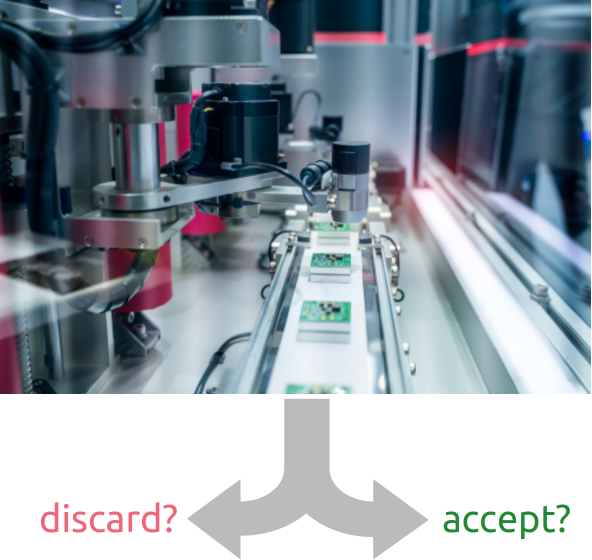
\includegraphics[width=1\textwidth,height=\textheight]{accept_discard.png}

}

\end{marginfigure}

{\textbf{\emph{Should the inspection device accept or discard the new
component?}}}\\

First, try to give and motivate an answer.

This is not the real question of this exercise, however. In fact it
doesn't matter if you don't get the correct answer; not even if you
don't manage to get an answer at all.

\begin{tcolorbox}[enhanced jigsaw, opacityback=0, colback=white, toprule=.15mm, left=2mm, colframe=quarto-callout-caution-color-frame, title={\faIcon{user-edit} Very first exercise!}, colbacktitle=quarto-callout-caution-color!10!white, leftrule=.75mm, rightrule=.15mm, opacitybacktitle=0.6, breakable, coltitle=black, bottomtitle=1mm, toptitle=1mm, titlerule=0mm, arc=.35mm, bottomrule=.15mm]

The purpose here is for you to do some introspection about your own
reasoning. Then examine and discuss these points:

\begin{itemize}
\item
  Which numerical elements in the problem seem to affect the answer?
\item
  Can these numerical elements be clearly separated? How would you
  separate them?
\item
  How would the answer change, if these numerical elements were changed?
  Feel free to change them, also in extreme ways, and see how the answer
  would change.
\item
  Could we solve the problem if we didn't have the probabilities? Why?
\item
  Could we solve the problem if we didn't know the various gains and
  losses? Why?
\item
  Can this problem be somehow abstracted, and then transformed into
  another one with completely different details? For instance, consider
  translating along these lines:

  \begin{itemize}
  \tightlist
  \item
    inspection device → computer pilot of self-driving car
  \item
    tests → camera image
  \item
    fail within a year → pedestrian in front of car
  \item
    accept/discard → keep on going/~break
  \end{itemize}
\end{itemize}

\end{tcolorbox}

\hypertarget{framework}{%
\chapter{Framework}\label{framework}}

\providecommand{\ul}{\uline}
\renewcommand*{\|}[1][]{\nonscript\:#1\vert\nonscript\:\mathopen{}}
\providecommand*{\pr}[1]{\textsf{\small`#1'}}
\renewcommand*{\pr}[1]{\textsf{\small`#1'}}
\providecommand*{\prq}[1]{\textsf{\small #1}}
\renewcommand*{\prq}[1]{\textsf{\small #1}}
\providecommand{\se}[1]{\mathsfit{#1}}
\renewcommand{\se}[1]{\mathsfit{#1}}
\providecommand{\p}{\mathrm{p}}
\renewcommand{\p}{\mathrm{p}}
\renewcommand{\P}{\mathrm{P}}
\definecolor{quarto-callout-note-color}{HTML}{4477AA}
\definecolor{quarto-callout-note-color-frame}{HTML}{4477AA}
\definecolor{quarto-callout-important-color}{HTML}{AA3377}
\definecolor{quarto-callout-important-color-frame}{HTML}{AA3377}
\definecolor{quarto-callout-warning-color}{HTML}{EE6677}
\definecolor{quarto-callout-warning-color-frame}{HTML}{EE6677}
\definecolor{quarto-callout-tip-color}{HTML}{228833}
\definecolor{quarto-callout-tip-color-frame}{HTML}{228833}
\definecolor{quarto-callout-caution-color}{HTML}{CCBB44}
\definecolor{quarto-callout-caution-color-frame}{HTML}{CCBB44}

\hypertarget{what-does-the-intro-problem-tell-us}{%
\section{What does the intro problem tell
us?}\label{what-does-the-intro-problem-tell-us}}

Let's approach the ``accept or discard?'' problem of the previous
chapter~\ref{sec-intro} in an intuitive way.

\marginnote{\begin{footnotesize}

We're jumping the gun here, because we haven't learned the method to
solve this problem yet!

\end{footnotesize}}

First let's say that we \texttt{accept} the component. What happens?

We must try to make sense of that \(10\%\) probability that the
component fails within a year. Different people do this with different
imagination tricks. We can imagine, for instance, that this situation is
repeated 100 times. In 10 of these repetitions the accepted electronic
component is sold and fails within a year after selling. In the
remaining 90 repetitions, the component is sold and works fine for at
least a year.

In each of the 10 imaginary repetitions in which the component fails
early, the manufacturer loses \(11\$\). That's a total loss of
\(10 \cdot 11\$ = 110\$\). In each of the 90 imaginary repetitions in
which the component doesn't fail early, the manufacturer gains \(1\$\).
That's a total gain of \(90\$\). So over all 100 imaginary repetitions
the manufacturer gains \[
10\cdot (-11\$) + 90\cdot 1\$ = {\color[RGB]{238,102,119} -20\$} \ ,
\] that is, the manufacturer has not gained, but \emph{lost} \(20\$\)\,!
That's an average of \(0.2\$\) \emph{lost} per repetition.

Now let's say that we \texttt{discard} the component instead. What
happens? In this case we don't need to invoke imaginary repetitions, but
even if we do, it's clear that the manufacturer doesn't gain or lose
anything -- that is, the ``gain'' is \(0\$\) -- in each and all of the
repetitions.

The conclusion is that if in a situation like this we {accept} the
component, then we'll {lose \(0.2\$\)} on average; whereas if we
{discard} it, then on average we won't {lose anything or gain anything}.

Obviously the best, or ``least worst'', decision to make is to
\textbf{discard} the component.

\begin{tcolorbox}[enhanced jigsaw, opacityback=0, colback=white, toprule=.15mm, left=2mm, colframe=quarto-callout-caution-color-frame, title={\faIcon{user-edit} Exercises}, colbacktitle=quarto-callout-caution-color!10!white, leftrule=.75mm, rightrule=.15mm, opacitybacktitle=0.6, breakable, coltitle=black, bottomtitle=1mm, toptitle=1mm, titlerule=0mm, arc=.35mm, bottomrule=.15mm]

\begin{enumerate}
\def\labelenumi{\arabic{enumi}.}
\item
  Now that we have an idea of the general reasoning, check what happens
  with different values of the probability of failure and of the failure
  cost: is it still best to discard? For instance, try with

  \begin{itemize}
  \tightlist
  \item
    failure probability \texttt{10\%} and failure cost \texttt{5\$};
  \item
    failure probability \texttt{5\%} and failure cost \texttt{11\$};
  \item
    failure probability \texttt{10\%}, failure cost \texttt{11\$},
    non-failure gain \texttt{2\$}.
  \end{itemize}

  Feel free to get wild and do plots.
\item
  Identify the failure probability at which accepting the component
  doesn't lead to any loss or any gain, so it doesn't matter whether we
  discard or accept. (You can solve this as you prefer: analytically
  with an equation, visually with a plot, by trial\,\&\,error on several
  cases, or whatnot.)
\item
  Consider the special case with failure probability \texttt{0\%} and
  failure cost \texttt{10\$}. This means no new component will ever
  fail. To decide in such a case we do not need imaginary repetitions;
  but \textbf{confirm} that we arrive at the same logical conclusion
  whether we reason through imaginary repetitions or not.
\item
  Consider this completely different problem:

  \begin{quote}
  A patient is examined by a brand-new medical diagnostics AI system.

  The AI first performs some clinical tests on the patient. The tests
  give an uncertain forecast of whether the patient has a particular
  disease or not.

  Then the AI decides whether the patient should be dismissed without
  treatment, or treated with a particular medicine.

  If the patient is dismissed, then the life expectancy doesn't increase
  or decrease if the disease is not present, but it decreases by
  10~years if the disease is actually present. If the patient is
  treated, then the life expectancy decreases by 1~year if the disease
  is not present (owing to treatment side-effects), but also if the
  disease is present (because it cures the disease, so the life
  expectancy doesn't decrease by 10 years; but it still decreases by 1
  year owing to the side effects).

  For this patient, the clinical tests indicate that there is a \(10\%\)
  probability that the patient has the disease.
  \end{quote}

  Should the diagnostic AI dismiss or treat the patient? Find
  differences and similarities, even numerical, with the assembly-line
  problem.
\end{enumerate}

\end{tcolorbox}

\hfill\break

From the solution of the problem and from the exploring exercises, we
gather some instructive points:

\begin{itemize}
\item
  Is it enough if we simply know that the component is less likely to
  fail than not? in other words, if we simply know that the probability
  of failure is less than \(50\%\)?

  Obviously not. We found that if the failure probability is \(10\%\)
  then it's best to discard; but if it's \(5\%\) then it's best to
  accept. In both cases the component was less likely to fail than not,
  but the decisions were different. Moreover, we found that the
  probability affected the loss if one made the non-optimal decision.
  Therefore:

  {\textbf{Knowledge of exact probabilities is absolutely necessary for
  making the best decision}}
\item
  Is it enough if we simply know that failure leads to a cost? that is,
  that its gain is less than the gain for non-failure?

  Obviously not. The situation is similar to that with the probability.
  In the exercise we found that if the failure cost is \(11\$\) then
  it's best to discard; but if it's \(5\$\) then it's best to accept.
  It's also best to accept if the failure cost is \(11\$\) but the
  non-failure gain is \(2\$\). Therefore:

  {\textbf{Knowledge of the exact gains and losses is absolutely
  necessary for making the best decision}}
\item
  Is this kind of decision situation only relevant to assembly lines and
  sales?

  By all means not. We found a clinical situation that's exactly
  analogous: there's uncertainty, there are gains and losses (of time
  rather than money), and the best decision depends on both.
\end{itemize}

\hypertarget{our-focus-decision-making-inference-and-data-science}{%
\section{Our focus: decision-making, inference, and data
science}\label{our-focus-decision-making-inference-and-data-science}}

Every data-driven engineering project is unique, with its unique
difficulties and problems. But there are also problems common to all
engineering projects.

In the scenarios we explored above, we found an extremely important
problem-pattern. There is a decision or choice to make (and ``not
deciding'' is not an option -- or it's just another kind choice). Making
a particular decision will lead to some consequences, some leading to a
desired goal, others leading to something undesirable. The decision is
difficult because its consequences are not known with certainty, given
the information and data available in the problem. We may lack
information and data about past or present details, about future events
and responses, and so on. This is what we call a problem of
{\textbf{decision-making under uncertainty}} or \textbf{under
risk}\footnote{We'll avoid the word ``risk'' because it has several
  different technical meanings in the literature, some even
  contradictory.}, or simply a ``decision problem'' for short.

This problem-pattern appears literally everywhere. But our explored
scenarios also suggest that this problem-pattern has a sort of
systematic solution method.

In this course we're going to focus on decision problems and their
systematic solution method. We'll learn a framework and some abstract
notions that allow us to frame and analyse this kind of problem, and
we'll learn a universal set of principles to solve it. This set of
principles goes under the name of {\textbf{Decision Theory}}.

But what do decision-making under uncertainty and Decision Theory have
to do with \emph{data} and \emph{data science}? The three are profoundly
and tightly related on many different planes:

\marginnote{\begin{footnotesize}

\begin{tcolorbox}[enhanced jigsaw, opacityback=0, colback=white, toprule=.15mm, left=2mm, colframe=quarto-callout-tip-color-frame, title={\faIcon{rocket} For the extra curious}, colbacktitle=quarto-callout-tip-color!10!white, leftrule=.75mm, rightrule=.15mm, opacitybacktitle=0.6, breakable, coltitle=black, bottomtitle=1mm, toptitle=1mm, titlerule=0mm, arc=.35mm, bottomrule=.15mm]

\href{https://hvl.instructure.com/courses/25074/modules/items/665981}{\emph{Decision
theory in expert systems and artificial intelligence}}

\end{tcolorbox}

\end{footnotesize}}

\begin{itemize}
\item
  We saw that \emph{probability} values are essential in a decision
  problem. How do we find them? As you can imagine, \emph{data} play an
  important part in their calculation. In our intro example, the failure
  probability must come from observations or experiments on similar
  electronic components.
\item
  We saw that also the values of \emph{gains and losses} are essential.
  \emph{Data} play an important part in their calculation as well.
\item
  \emph{Data science} is based on the laws of \emph{Decision Theory}.
  Here's an analogy: a rocket engineer relies on fundamental physical
  laws (balance of momentum, energy, and so on) for making a rocket
  work. Failure to account for those laws leads at best to sub-optimal
  solutions, at worst to disasters. As we shall see, the same is true
  for a data scientist and the rules of decision theory.
\item
  \emph{Machine-learning} algorithms, in particular, are realizations or
  approximations of the rules of \emph{Decision Theory}. This is clear,
  for instance, considering that the main task of a machine-learning
  classifier is to decide among possible output labels or classes.
\item
  The rules of \emph{Decision Theory} are also the foundations upon
  which \emph{artificial-intelligence} agents, which must make optimal
  inferences and decisions, are built.
\end{itemize}

These five planes will constitute the major parts of the present course.

\hfill\break

@@ TODO add examples: algorithm giving outputs is a decision agent.

There are other important aspects in engineering problems, besides the
one of making decisions under uncertainty. For instance the
\emph{discovery} or the \emph{invention} of new technologies and
solutions. These aspects can barely be planned or decided; but their
fruits, once available, should be handled and used optimally -- thus
leading to a decision problem.

Artificial intelligence is proving to be a valuable aid in these more
creative aspects too. This kind of use of AI is outside the scope of the
present notes. Some aspects of this creativity-assisting use, however,
do fall within the domain of the present notes. A pattern-searching
algorithm, for example, can be optimized by means of the method we are
going to study.

\hypertarget{our-goal-optimality-not-success}{%
\section{Our goal: optimality, not
``success''}\label{our-goal-optimality-not-success}}

What should we demand from a systematic method for solving decision
problems?

By definition, in a decision problem under uncertainty there is
generally no method to \emph{determine} the decision that surely leads
to the desired consequence -- if such a method existed, then the problem
would not have any uncertainty! Therefore, if there is a method to deal
with decision problems, its goal cannot be the determination of the
\emph{successful} decision. This also means that a priori we cannot
blame an engineer for making an unsuccessful decision in a situation of
uncertainty.

Imagine two persons, Henry and Tina, who must bet on ``heads'' or
``tails'' under the following conditions (but who otherwise don't get
any special thrill from betting):

\begin{itemize}
\tightlist
\item
  If the bet is ``heads'' and the coin lands ``heads'', the person wins
  a \emph{small} amount of money; but if it lands ``tails'', they lose a
  \emph{large} amount of money.
\item
  If the bet is ``tails'' and the coin lands ``tails'', the person
  \emph{wins} a small amount of money; if it lands ``heads'', they lose
  the same \emph{small} amount of money.
\end{itemize}

Henry chooses the first bet, on ``heads''. Tina chooses the second bet,
on ``tails''. The coin comes down ``heads''. So Henry wins the small
amount of money, while Tina loses the same small amount. What would we
say about their decisions?

Henry's decision was lucky, and yet \emph{irrational}: he risked losing
much more money than in the second bet, without any possibility of at
least winning more. Tina's decision was unlucky, and yet
\emph{rational}: the possibility and amount of winning was the same in
the two bets, and she chose the bet with the least amount of loss. We
expect that any person making Henry's decision in similar, future bets
will eventually lose more money than any person making Tina's decision.

This example shows two points. First, ``success'' is generally not a
good criterion to judge a decision under uncertainty; success can be the
pure outcome of luck, not of smarts. Second, even if there is no method
to determine which decision is successful, there is a method to
determine which decision is rational or {\textbf{optimal}}, given the
particular gains, losses, and uncertainties involved in the decision
problem. We had a glimpse of this method in our introductory scenarios.

Let us emphasize, however, that we are not giving up on ``success'', or
trading it for ``optimality''. Indeed we'll find that {\textbf{Decision
Theory automatically leads to the \emph{successful} decision}} in
problems where uncertainty is not present or is irrelevant. It's a
win-win. It's important to keep this point in mind:

\begin{figure*}

\begin{tcolorbox}[enhanced jigsaw, opacityback=0, colback=white, toprule=.15mm, left=2mm, colframe=quarto-callout-note-color-frame, title={}, colbacktitle=quarto-callout-note-color!10!white, leftrule=.75mm, rightrule=.15mm, opacitybacktitle=0.6, breakable, coltitle=black, bottomtitle=1mm, toptitle=1mm, titlerule=0mm, arc=.35mm, bottomrule=.15mm]

{Aiming to find the solutions that are \emph{successful} can make us
\emph{fail} to find those that are optimal when the successful ones
cannot be determined.}

{Aiming to find the solutions that are \emph{optimal} makes us
automatically find those that are \emph{successful} when those can be
determined.}

\end{tcolorbox}

\end{figure*}

We shall later witness this fact with our own eyes, and will take it up
again in the discussion of some misleading techniques to evaluate
machine-learning algorithms.

\hypertarget{decision-theory}{%
\section{Decision Theory}\label{decision-theory}}

So far we have mentioned that Decision Theory has the following
features:

\begin{itemize}
\item
  {\faIcon{check} it tells us what's optimal and, when possible, what's
  successful}
\item
  {\faIcon{check} it takes into consideration decisions, consequences,
  costs and gains}
\item
  {\faIcon{check} it is able to deal with uncertainties}
\end{itemize}

What other kinds of features should we demand from it, in order to be
applied to as many kinds of decision problems as possible, and to be
relevant for data science?

If we find an optimal decision in regards to some outcome, it may still
happen that the decision can be realized in several ways that are
equivalent in regard to the outcome, but inequivalent in regard to time
or resources. In the assembly-line scenario, for example, the decision
\texttt{discard} could be carried out by burning, recycling, and so on.
We thus face a decision within a decision. In general, a decision
problem may involve several decision sub-problems, in turn involving
decision sub-sub-problems, and so on.

In data science, a common engineering goal is to design and build an
automated or AI-based device capable of making an optimal decision in a
specific kind of uncertain situations. Think for instance of an
aeronautic engineer designing an autopilot system, or a software company
designing an image classifier.

Decision Theory turns out to meet these demands too, thanks to the
following features:

\begin{itemize}
\item
  {\faIcon{check} it is susceptible to recursive, sequential, and
  modular application}
\item
  {\faIcon{check} it can be used not only for human decision-makers, but
  also for automated or AI devices}
\end{itemize}

\hfill\break

Decision Theory has a long history, going back to Leibniz in the 1600s
and partly even to Aristotle in the −300s, and appearing in its present
form around 1920--1960. What's remarkable about it is that it is not
only \emph{a} framework, but \emph{the} framework we must use. A
logico-mathematical theorem shows that {\textbf{any framework that does
not break basic optimality and rationality criteria has to be equivalent
to Decision Theory}}. In other words, any ``alternative'' framework may
use different technical terminology and rewrite mathematical operations
in a different way, but it boils down to the same notions and operations
of Decision Theory. So if you wanted to invent and use another
framework, then either (a) it would lead to some irrational or illogical
consequences, or (b) it would lead to results identical to Decision
Theory's. Many frameworks that you are probably familiar with, such as
optimization theory or Boolean logic, are just specific applications or
particular cases of Decision Theory.

Thus we list one more important characteristic of Decision Theory:

\begin{itemize}
\tightlist
\item
  {\faIcon{check} it is {\textbf{normative}}}
\end{itemize}

\marginnote{\begin{footnotesize}

\begin{tcolorbox}[enhanced jigsaw, opacityback=0, colback=white, toprule=.15mm, left=2mm, colframe=quarto-callout-tip-color-frame, title={\faIcon{rocket} For the extra curious}, colbacktitle=quarto-callout-tip-color!10!white, leftrule=.75mm, rightrule=.15mm, opacitybacktitle=0.6, breakable, coltitle=black, bottomtitle=1mm, toptitle=1mm, titlerule=0mm, arc=.35mm, bottomrule=.15mm]

\begin{itemize}
\tightlist
\item
  \href{https://hvl.instructure.com/courses/25074/modules/items/665858}{\emph{Judgment
  under uncertainty}}
\item
  \href{https://hvl.instructure.com/courses/25074/modules/items/665859}{\emph{Heuristics
  and Biases}}
\item
  \href{https://hvl.instructure.com/courses/25074/modules/items/665860}{\emph{Thinking,
  Fast and Slow}}
\end{itemize}

\end{tcolorbox}

\end{footnotesize}}

\emph{Normative} contrasts with \emph{descriptive}. The purpose of
Decision Theory is not to describe, for example, how human
decision-makers typically make decisions. Because human decision-makers
typically make irrational, sub-optimal, or biased decisions. That's
exactly what we want to avoid and improve!

\hypertarget{basic-decision-problems}{%
\chapter{Basic decision problems}\label{basic-decision-problems}}

\providecommand{\ul}{\uline}
\renewcommand*{\|}[1][]{\nonscript\:#1\vert\nonscript\:\mathopen{}}
\providecommand*{\pr}[1]{\textsf{\small`#1'}}
\renewcommand*{\pr}[1]{\textsf{\small`#1'}}
\providecommand*{\prq}[1]{\textsf{\small #1}}
\renewcommand*{\prq}[1]{\textsf{\small #1}}
\providecommand{\se}[1]{\mathsfit{#1}}
\renewcommand{\se}[1]{\mathsfit{#1}}
\providecommand{\p}{\mathrm{p}}
\renewcommand{\p}{\mathrm{p}}
\renewcommand{\P}{\mathrm{P}}
\definecolor{quarto-callout-note-color}{HTML}{4477AA}
\definecolor{quarto-callout-note-color-frame}{HTML}{4477AA}
\definecolor{quarto-callout-important-color}{HTML}{AA3377}
\definecolor{quarto-callout-important-color-frame}{HTML}{AA3377}
\definecolor{quarto-callout-warning-color}{HTML}{EE6677}
\definecolor{quarto-callout-warning-color-frame}{HTML}{EE6677}
\definecolor{quarto-callout-tip-color}{HTML}{228833}
\definecolor{quarto-callout-tip-color-frame}{HTML}{228833}
\definecolor{quarto-callout-caution-color}{HTML}{CCBB44}
\definecolor{quarto-callout-caution-color-frame}{HTML}{CCBB44}

Decision Theory analyses any decision-making problem in terms of nested
or sequential \emph{basic} or \emph{minimal} decision problems. The
assembly-line scenario of the introduction~\ref{sec-intro} is an
example.

\hypertarget{graphical-representation-and-elements}{%
\section{Graphical representation and
elements}\label{graphical-representation-and-elements}}

A basic decision problem can be represented by a diagram like this:

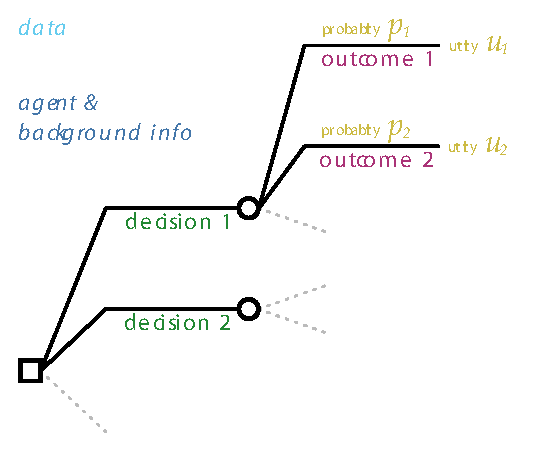
\includegraphics[width=1\textwidth,height=\textheight]{index_files/mediabag/basic_decision_tree.pdf}

It has one \emph{decision node}, usually represented by a square
\faIcon{square}, from which the available decisions depart as lines.
Each decision leads to an \emph{uncertainty node}, usually represented
by a circle \faIcon{circle}, from which the possible outcomes depart as
lines. Each outcome leads to a particular utility value. The uncertainty
of each outcome is quantified by a probability.

A basic decision problem is analysed in terms of these elements:

\begin{itemize}
\tightlist
\item
  {\faIcon{cube} \textbf{Agent}}, and {\textbf{background}} or
  {\textbf{prior information}}. The agent is the person or device that
  has to make the decision. An agent always possess (or has been
  programmed with) specific background information that is used and
  taken for granted in the decision-making process. This background
  information determines the probabilities and utilities of the
  outcomes, together with other available data and information. Since
  different agents typically have different background information, we
  shall somehow conflate agents and prior information.
\end{itemize}

\marginnote{\begin{footnotesize}

We'll use the neutral pronouns \emph{it}/\emph{its} when referring to an
agent, since an agent could be a person or a machine.

\end{footnotesize}}

\begin{itemize}
\item
  {\faIcon{cube} \textbf{Decisions}}, also called \textbf{courses of
  actions}, available to the agent. They are assumed to be mutually
  exclusive and exhaustive; this can always be achieved by recombining
  them if necessary, as we'll discuss later.
\item
  {\faIcon{cube} \textbf{Outcomes}} of the possible decisions. Every
  decision can have a different set of outcomes, or some outcomes can
  appear for several or all decisions (in this case they are reported
  multiple times in the decision diagram). Note that even if an outcome
  can happen for two or more different decisions, its probabilities can
  still be different depending on the decision.
\item
  {\faIcon{cube} \textbf{Probabilities}} for each of the outcomes. Their
  values typically depend on the background information, the decision,
  and the additional data.
\item
  {\faIcon{cube} \textbf{Utilities}}: the gains or losses associated
  with each of the possible outcomes. Their values also depend on the
  background information, the decision, and the additional data.
\item
  {\faIcon{cube} \textbf{Data}} and other {\textbf{additional
  information}}, sometimes called {\textbf{evidence}}. They differ from
  the background information in that they can change with every decision
  instance made by the same agent, while the background information
  stays the same. In the assembly-line scenario, for example, the test
  results could be different for every new electric component.
\end{itemize}

\marginnote{\begin{footnotesize}

\begin{tcolorbox}[enhanced jigsaw, opacityback=0, colback=white, toprule=.15mm, left=2mm, colframe=quarto-callout-tip-color-frame, title={}, colbacktitle=quarto-callout-tip-color!10!white, leftrule=.75mm, rightrule=.15mm, opacitybacktitle=0.6, breakable, coltitle=black, bottomtitle=1mm, toptitle=1mm, titlerule=0mm, arc=.35mm, bottomrule=.15mm]

\faIcon{seedling} Remember: What matters is to be able to identify these
elements in a concrete problem, understanding their role. Their
technical names don't matter.

\end{tcolorbox}

\end{footnotesize}}

Note that it is not always the case that the \emph{outcomes} are unknown
and the \emph{data} are known. As we'll discuss later, in some
situations we reason in hypothetical or counterfactual ways, using
hypothetical data and considering outcomes which have already occurred.

\begin{tcolorbox}[enhanced jigsaw, opacityback=0, colback=white, toprule=.15mm, left=2mm, colframe=quarto-callout-caution-color-frame, title={\faIcon{book} Reading}, colbacktitle=quarto-callout-caution-color!10!white, leftrule=.75mm, rightrule=.15mm, opacitybacktitle=0.6, breakable, coltitle=black, bottomtitle=1mm, toptitle=1mm, titlerule=0mm, arc=.35mm, bottomrule=.15mm]

§\,1.1.4 in
\href{https://hvl.instructure.com/courses/25074/modules/items/660089}{\emph{Artificial
Intelligence}}

\end{tcolorbox}

\begin{tcolorbox}[enhanced jigsaw, opacityback=0, colback=white, toprule=.15mm, left=2mm, colframe=quarto-callout-caution-color-frame, title={\faIcon{user-edit} Exercise}, colbacktitle=quarto-callout-caution-color!10!white, leftrule=.75mm, rightrule=.15mm, opacitybacktitle=0.6, breakable, coltitle=black, bottomtitle=1mm, toptitle=1mm, titlerule=0mm, arc=.35mm, bottomrule=.15mm]

\begin{itemize}
\tightlist
\item
  Identify the elements above in the assembly-line decision problem of
  the introduction~\ref{sec-intro}.
\item
  Sketch the diagram of the assembly-line decision problem.
\end{itemize}

\end{tcolorbox}

Some of the decision-problem elements listed above may need to be in
turn analysed by a decision sub-problem. For instance, the utilities
could depend on uncertain factors: thus we have a decision sub-problem
to determine the optimal values to be used for the utilities of the main
problem. This is an example of the modular character of decision theory.

We shall soon see how to mathematically represent these elements.

The elements above must be identified unambiguously in every decision
problem. The analysis into these elements greatly helps in making the
problem and its solution well-defined.

An advantage of decision theory is that its application \emph{forces} us
to make sense of an engineering problem. A useful procedure is to
formulate the general problem in terms of the elements above,
identifying them clearly. If the definition of any of the terms involves
uncertainty of further decisions, then we analyse it in turn as a
decision sub-problem, and so on.

\begin{quote}
Suppose someone (probably a politician) says: ``We must solve the energy
crisis by reducing energy consumption or producing more energy''. From a
decision-making point of view, this person has effectively said
\emph{nothing whatsoever}. By definition the ``energy crisis'' is the
problem that energy production doesn't meet demand. So this person has
only said ``we would like the problem to be solved'', without specifying
any solution. A decision-theory approach to this problem requires us to
specify which concrete courses of action should be taken for reducing
consumption or increasing productions, and what their probable outcomes,
costs, and gains would be.
\end{quote}

\marginnote{\begin{footnotesize}

\begin{tcolorbox}[enhanced jigsaw, opacityback=0, colback=white, toprule=.15mm, left=2mm, colframe=quarto-callout-tip-color-frame, title={\faIcon{rocket} For the extra curious}, colbacktitle=quarto-callout-tip-color!10!white, leftrule=.75mm, rightrule=.15mm, opacitybacktitle=0.6, breakable, coltitle=black, bottomtitle=1mm, toptitle=1mm, titlerule=0mm, arc=.35mm, bottomrule=.15mm]

See MacKay's options-vs-costs rational analysis in
\href{https://www.withouthotair.com}{Sustainable Energy -- without the
hot air}

\end{tcolorbox}

\end{footnotesize}}

\hypertarget{inference-utility-maximization}{%
\section{Inference, utility,
maximization}\label{inference-utility-maximization}}

The solution of a basic decision-making problem can be roughly divided
into three main stages: inference, utility assessment, and
expected-utility maximization.

{\faIcon{cube} \textbf{Inference}} is the stage where the probabilities
of the possible outcomes are calculated. Its rules are given by the
{\textbf{Probability Calculus}}. Inference is independent from decision:
in some situations we may simply wish to assess whether some hypotheses,
conjectures, or outcomes are more or less plausible than others, without
making any decision. This kind of assessment can be very important in
problems of communication and storage, and it is specially considered by
{\textbf{Information Theory}}.

The calculation of probabilities can be the part that demands most
thinking, time, and computational resources in a decision problem. It is
also the part that typically makes most use of data -- and where data
can be most easily misused.

Roughly half of this course will be devoted in understanding the laws of
inference, their applications, uses, and misuses.\\

{\faIcon{cube} \textbf{Utility assesment}} is the stage where the gains
or losses of the possible outcomes are calculated. Often this stage
requires further inferences and further decision-making sub-problems.
The theory underlying utility assessment is still much underdeveloped,
compared to probability theory.\\

{\faIcon{cube} \textbf{Expected-utility maximization}} is the final
stage where the probabilities and gains or costs of the possible
outcomes are combined, in order to determine the optimal decision.

\part{Inference}

\hypertarget{inference-1}{%
\chapter{Inference}\label{inference-1}}

\providecommand{\ul}{\uline}
\renewcommand*{\|}[1][]{\nonscript\:#1\vert\nonscript\:\mathopen{}}
\providecommand*{\pr}[1]{\textsf{\small`#1'}}
\renewcommand*{\pr}[1]{\textsf{\small`#1'}}
\providecommand*{\prq}[1]{\textsf{\small #1}}
\renewcommand*{\prq}[1]{\textsf{\small #1}}
\providecommand{\se}[1]{\mathsfit{#1}}
\renewcommand{\se}[1]{\mathsfit{#1}}
\providecommand{\p}{\mathrm{p}}
\renewcommand{\p}{\mathrm{p}}
\renewcommand{\P}{\mathrm{P}}
\definecolor{quarto-callout-note-color}{HTML}{4477AA}
\definecolor{quarto-callout-note-color-frame}{HTML}{4477AA}
\definecolor{quarto-callout-important-color}{HTML}{AA3377}
\definecolor{quarto-callout-important-color-frame}{HTML}{AA3377}
\definecolor{quarto-callout-warning-color}{HTML}{EE6677}
\definecolor{quarto-callout-warning-color-frame}{HTML}{EE6677}
\definecolor{quarto-callout-tip-color}{HTML}{228833}
\definecolor{quarto-callout-tip-color-frame}{HTML}{228833}
\definecolor{quarto-callout-caution-color}{HTML}{CCBB44}
\definecolor{quarto-callout-caution-color-frame}{HTML}{CCBB44}

In the assembly-line decision problem of §~\ref{sec-intro}, the
probability of early failure (and that of late failure), in view of the
test results, was very important in determining the optimal decision. If
the probability had been \(5\%\) instead of \(10\%\), the optimal
decision would have been different. In that scenario the probabilities
of the outcomes in view of the test results were already given. In real
decision problems, however, probabilities almost always need to be
calculated, and their calculation can be the most time- and
resource-demanding step in solving a decision problem.

We'll loosely refer to problems of calculating probabilities as
``\emph{inference} problems'', and to their calculation as ``drawing an
inference''. Drawing inferences is very often a goal or need in itself,
with no underlying decision process. Let's see a couple more informal
examples of inference problems before continuing; for some of them an
underlying decision problem is also alluded to:

\begin{enumerate}
\def\labelenumi{\Alph{enumi}.}
\item
  Looking at the weather we try to assess if it'll rain today, to decide
  whether to take an umbrella.
\item
  Considering a patient's symptoms, test results, and medical history, a
  clinician tries to assess which disease affects a patient, so as to
  decide on the optimal treatment.
\item
  Looking at the present game position
  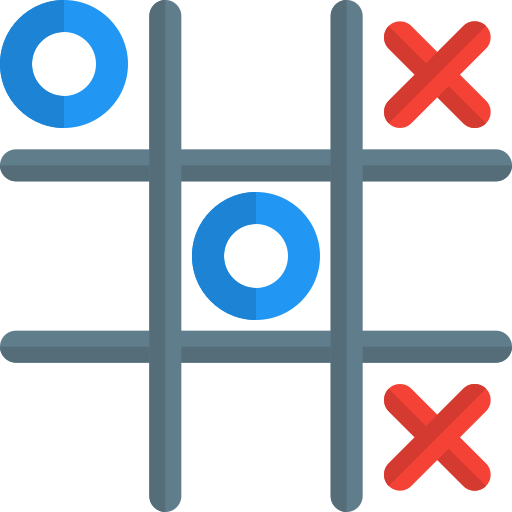
\includegraphics[width=0.1\textwidth,height=\textheight]{XsOs.png} the
  X-player, which moves next, wonders whether placing the next
  {\textbf{X}} on the mid-right position leads to a win.
\item
  From the current set of camera frames, the computer of a self-driving
  car needs to assess whether a particular patch of colours in the
  frames is a person, so as to slow down the car and stop.
\item
  Given that {\(G=6.67 \cdot 10^{-11}\,\mathrm{m^3\,s^{-2}\,kg^{-1}}\),}
  \(M = 5.97 \cdot 10^{24}\,\mathrm{kg}\) (mass of the Earth), and
  \(r = 6.37 \cdot 10^{6}\,\mathrm{m}\) (radius of the Earth),
  \href{http://nasaphysics.cet.edu/escape-velocity.html}{a rocket
  engineer needs to know} how much is {\(\sqrt{2\,G\,M/r\,}\).}
\item
  We'd like to know whether the rolled die is going to show
  \faIcon{dice-six}.
\item
  An
  \href{https://aerospaceamerica.aiaa.org/features/a-i-in-the-cockpit}{aircraft's
  autopilot system} needs to assess how much the aircraft's
  \href{https://www.grc.nasa.gov/www/k-12/VirtualAero/BottleRocket/airplane/roll.html}{roll}
  will change if the right wing's
  \href{https://www.grc.nasa.gov/www/k-12/VirtualAero/BottleRocket/airplane/incline.html}{angle
  of attack} is increased by \(0.1\,\mathrm{rad}\).
\item
  By looking at the dimensions, shape, texture of a newly dug-out fossil
  bone, an archaeologist wonders whether it belonged to a Tyrannosaurus
  rex.
\item
  A voltage test on a newly produced electronic component yields a
  reading of \(100\,\mathrm{mV}\). The electronic component turns out to
  be defective. An engineer wants to assess whether the voltage-test
  reading could have been \(100\,\mathrm{mV}\), if the component had not
  been defective.
\item
  Same as above, but the engineer wants to assess whether the
  voltage-test reading could have been \(80\,\mathrm{mV}\), if the
  component had not been defective.
\end{enumerate}

\begin{tcolorbox}[enhanced jigsaw, opacityback=0, colback=white, toprule=.15mm, left=2mm, colframe=quarto-callout-caution-color-frame, title={\faIcon{user-edit} Exercises}, colbacktitle=quarto-callout-caution-color!10!white, leftrule=.75mm, rightrule=.15mm, opacitybacktitle=0.6, breakable, coltitle=black, bottomtitle=1mm, toptitle=1mm, titlerule=0mm, arc=.35mm, bottomrule=.15mm]

\begin{enumerate}
\def\labelenumi{\arabic{enumi}.}
\setcounter{enumi}{4}
\item
  For each example above, pinpoint what has to be inferred.
\item
  Point out which of the examples above \emph{explicitly} gives data or
  information that should be used for the inference.
\item
  For the examples that do not give explicit data or information,
  speculate what information could be implicitly assumed. For those that
  do give explicit data, speculate which other additional information
  could be implicitly assumed.
\item
  Can any of the inferences above be done perfectly, that is, without
  any uncertainty (from the data given explicitly or implicitly)?
\item
  Point out which of the examples above explicitly involves a decision.
\item
  For the examples that involve a decision: in which of them does the
  decision affect the results of the inference? In which it does not?
\item
  Point out which of the inferences above is about something that could
  be already known, at least in theory (for instance something that
  already happened).
\item
  Are any of the inferences above about something that is actually
  already known?
\item
  Are any of the inferences above about something that actually did not
  happen?
\item
  Do any of the inferences above use ``data'' or ``information'' that
  are actually not real (and are known not to be real)?
\end{enumerate}

\end{tcolorbox}

How are inference problems solved? We shall learn a universal set of
principles to solve them, called the {\textbf{probability calculus}} or
more commonly \textbf{probability theory}\footnote{We'll soon see why
  ``calculus'' is a more appropriate name than ``theory''.}

We now put momentarily the full decision-making problem backstage (but
keeping it in the back of our minds), and focus on the problem of
{\textbf{inference}}. Drawing inferences is very often a goal or need in
itself, with no underlying decision process.

\hypertarget{what-is-inference}{%
\section{What is inference?}\label{what-is-inference}}

\emph{Drawing an inference} could mean: to assess whether an unknown
outcome or hypothesis is \texttt{true} or \texttt{false}, on the basis
of some known data and information. This definition, however, is too
limited in two respects, especially in problems of engineering and data
science. We need to make it more general:

\hypertarget{from-truth-to-probability}{%
\subsection{From truth to probability}\label{from-truth-to-probability}}

Our starting point is decision-making \emph{under uncertainty}, because
in concrete engineering problems it is often impossible to determine the
truth or falsity of a hypothesis with certainty.

So by \emph{drawing an inference} we cannot mean {\textbf{to assess the
plausibility}} or {\textbf{credibility}} or {\textbf{probability}}
rather than the truth or falsity. Truth-determination is still included
as a special case: \texttt{fully\ certain} corresponds to \texttt{true},
and \texttt{impossible} corresponds to \texttt{false}. We'll discuss the
``plausibility'' idea in more detail later.

\hypertarget{hypothetical-and-counterfactual-inferences}{%
\subsection{Hypothetical and counterfactual
inferences}\label{hypothetical-and-counterfactual-inferences}}

It is not always the case that we want to assess the truth or
plausibility of something \emph{unknown} on the basis of something
\emph{known}. An agent must often make \textbf{hypothetical} or
\textbf{counterfactual} reasoning.

Our assembly-line scenario gives a concrete example. The inference there
is that the component will fail within a year \emph{if} it is accepted
and sold. But that hasn't been decided yet; maybe it's going to be
rejected instead. This is an example of \emph{hypothetical reasoning}:
we are making an inference based partly on facts and partly on imagined
information, whose truth is still unknown.

In other situations, for example when backtracking an error, we may need
to assess the plausibility of an outcome which did \emph{not} happen,
based on a hypothesis which may or may not be true. This assessment may
help us in ruling out that hypothesis. This is an example of
\emph{counterfactual reasoning}.

Both these kinds of reasoning are staples of scientific research. We
will see that they continuously enter in the calculation of
probabilities.

\hypertarget{proposal-and-conditional}{%
\section{Proposal and conditional}\label{proposal-and-conditional}}

\hfill\break

Some additional aspects of inference must be emphasized:

\hypertarget{known-and-unknown-by-whom}{%
\subsection{Known and unknown: by
whom?}\label{known-and-unknown-by-whom}}

What's known to an agent can be unknown to another agent, and vice
versa. This means that {\textbf{every inference is always relative to an
agent's background knowledge}}. This fact is especially important in
data science and artificial intelligence.

Consider an engineer testing the programming of a particular AI system.
The engineer inputs specially-chosen data and checks the AI's decisions
about specially-chosen outcomes. In this scenario we have two ongoing
inferences, drawn by two agents:

\begin{itemize}
\item
  The AI is one agent. This agent knows the inputs, but doesn't know the
  true outcomes. This agent's inference is about the outcomes.
\item
  The engineer is the other agent. This agent knows inputs and true
  outcomes -- both are ``data'' for this agent -- but doesn't know the
  AI's final decisions. This agent's inference is about the AI's
  decisions.
\end{itemize}

\hypertarget{future-and-past}{%
\subsection{Future and past}\label{future-and-past}}

An inference may concern not only unknown future outcomes,\footnote{an
  inference about the future is often called a \emph{forecast}.} but
also unknown \emph{past} outcomes. For instance, imagine that a
particular device has stopped working, and an engineer needs to assess
the plausibility that a mechanical failure happened, or an electronic
failure happened. In this case the inference is about something unknown
to the engineer (and maybe to anyone else), but that has already
happened. Astrophysicists and archaeologists draw this kind of
inferences all the time.

\hypertarget{mathematical-representation-of-inferences-and-their-objects}{%
\section{Mathematical representation of inferences and their
objects}\label{mathematical-representation-of-inferences-and-their-objects}}

We shall soon explore the rules that govern inference. But first we must
address two questions:

\begin{itemize}
\item
  Inference \emph{about what}? and \emph{given what}? So far we've
  spoken about ``outcomes'', ``data'', ``hypotheses'', ``background
  knowledge'', and similar concepts. They are not identical concepts;
  can we view them all as instances of a more unified notion?
\item
  How to mathematically \emph{represent} this unified notion and those
  concepts? A mathematical representation is necessary for
  systematically approaching inference and decision problems of any
  complexity, and also for implementation in computer algorithms and
  artificial-intelligence agents.
\end{itemize}

\hypertarget{sentences}{%
\chapter{Sentences}\label{sentences}}

\providecommand{\ul}{\uline}
\renewcommand*{\|}[1][]{\nonscript\:#1\vert\nonscript\:\mathopen{}}
\providecommand*{\pr}[1]{\textsf{\small`#1'}}
\renewcommand*{\pr}[1]{\textsf{\small`#1'}}
\providecommand*{\prq}[1]{\textsf{\small #1}}
\renewcommand*{\prq}[1]{\textsf{\small #1}}
\providecommand{\se}[1]{\mathsfit{#1}}
\renewcommand{\se}[1]{\mathsfit{#1}}
\providecommand{\p}{\mathrm{p}}
\renewcommand{\p}{\mathrm{p}}
\renewcommand{\P}{\mathrm{P}}
\definecolor{quarto-callout-note-color}{HTML}{4477AA}
\definecolor{quarto-callout-note-color-frame}{HTML}{4477AA}
\definecolor{quarto-callout-important-color}{HTML}{AA3377}
\definecolor{quarto-callout-important-color-frame}{HTML}{AA3377}
\definecolor{quarto-callout-warning-color}{HTML}{EE6677}
\definecolor{quarto-callout-warning-color-frame}{HTML}{EE6677}
\definecolor{quarto-callout-tip-color}{HTML}{228833}
\definecolor{quarto-callout-tip-color-frame}{HTML}{228833}
\definecolor{quarto-callout-caution-color}{HTML}{CCBB44}
\definecolor{quarto-callout-caution-color-frame}{HTML}{CCBB44}

\hypertarget{data-outcomes-agents-decisions}{%
\section{Data, outcomes, agents,
decisions}\label{data-outcomes-agents-decisions}}

Is there a flexible and general way of representing data, outcomes,
background information, hypotheses, assumptions, and even decisions?

When speaking of ``data'', what comes to mind to many people is
basically numbers or collections of numbers. Maybe numbers, then, could
be used to represent all the concepts above. This possibility turns out
to be too restricting.

I give you this number: {``\(8\)'',} saying that it is ``data''. But
what is it about? You, as an agent, can hardly call this number a piece
of information, because you have no clue what to do with it. Instead, if
I tell you: ``\href{https://solarsystem.nasa.gov/planets/overview}{The
number of official planets in the solar system is 8}'', then we can say
that I've given you data. So ``data'' is not just numbers: a number is
not ``data'' unless there's an additional verbal, non-numeric context
accompanying it, even if only implicitly. Sure, we could represent this
meta-data information as numbers too; but this move would only shift the
problem one level up: we would need an auxiliary verbal context
explaining what the meta-data numbers are about.

Data can, moreover, be completely non-numeric. A clinician saying ``The
patient has fully recovered from the disease'' (we imagine to know who's
the patient and what was the disease) is giving us a piece of
information that we could further use, for instance, to make prognoses
about other, similar patients. The clinician's statement surely is
``data'', but essentially non-numeric data. In some situations we can
represent it as ``1'', while ``0'' would represent ``not recovered''.
Yet the opposite convention could also be used, showing that these two
numbers have intrinsically nothing to do with the clinician's data.

But the examples above actually reveal the answer to our needs. In the
examples we expressed the data by means of \emph{sentences}. Clearly any
piece of information, outcome, hypothesis, decision can be expressed by
a sentence. We shall therefore use {\textbf{sentences}}, also called
\textbf{propositions} or \textbf{statements},\footnote{These three terms
  are not always equivalent in formal logic, but here we'll use them as
  synonyms.} to represent and communicate background information, data,
outcomes, hypotheses, knowns, unknowns, and any other things on which or
from which inferences can be drawn. In some cases we can of course
summarize a sentence by a number, as a shorthand, when the full meaning
of the sentence is understood.

But what is a sentence, more exactly? The everyday meaning of this word
will work for us, even though there is still a lot of research in logic
an artificial intelligence on how to define and use sentences. We shall
adopt this useful definition:

\marginnote{\begin{footnotesize}

\begin{tcolorbox}[enhanced jigsaw, opacityback=0, colback=white, toprule=.15mm, left=2mm, colframe=quarto-callout-tip-color-frame, title={\faIcon{rocket} For the extra curious}, colbacktitle=quarto-callout-tip-color!10!white, leftrule=.75mm, rightrule=.15mm, opacitybacktitle=0.6, breakable, coltitle=black, bottomtitle=1mm, toptitle=1mm, titlerule=0mm, arc=.35mm, bottomrule=.15mm]

\href{https://plato.stanford.edu/archives/win2020/entries/propositions}{Propositions}

\end{tcolorbox}

\end{footnotesize}}

\begin{tcolorbox}[enhanced jigsaw, opacityback=0, colback=white, toprule=.15mm, left=2mm, colframe=quarto-callout-note-color-frame, title={}, colbacktitle=quarto-callout-note-color!10!white, leftrule=.75mm, rightrule=.15mm, opacitybacktitle=0.6, breakable, coltitle=black, bottomtitle=1mm, toptitle=1mm, titlerule=0mm, arc=.35mm, bottomrule=.15mm]

{A ``sentence'' is a verbal message for which we can determine whether
it is \texttt{true} or \texttt{false}, at least in principle and in such
a way that all interested receivers of the message would agree.}

\end{tcolorbox}

For instance, in most engineering contexts the phrase ``This valve will
operate for at least two months'' is a sentence; whereas the phrase
``Apples are much tastier than pears'' is not, because it's a matter of
personal taste -- there's no objective criterion to determine its truth
or falsity. However, the phrase ``Rita finds apples tastier than pears''
could be a sentence (its truth is found by asking Rita).

\marginnote{\begin{footnotesize}

We shall see later that a phrase may contain a lot of technical terms,
and still not be a sentence.

\end{footnotesize}}

Note that a sentence can contain numbers, and even \emph{pictures and
graphs}: this possibility is not excluded from the definition above.

The use of sentences in our framework has important practical
consequences:

\begin{itemize}
\item
  \textbf{Clarity, analysis, goal-orientation}. A data engineer must
  acquire information and convey information. ``Acquiring information''
  does not simply consist in making measurements or counting something:
  the engineer must understand \emph{what} is being measured and
  \emph{why}. If data is gathered from third parties, the engineer must
  ask what exactly the data mean and how they were acquired. In
  designing and engineering a solution, it is important to understand
  what information or outcomes the end user exactly wants. A data
  engineer will often ask ``\emph{wait, what do you mean by that?}''.
  This question is not just an unofficial parenthesis in the official
  data-transfer workflow between the engineer and someone else. It is an
  integral part of that workflow: it means that some data have not been
  completely transferred yet.
\item
  \textbf{Artificial Intelligence}. Sentences are the central components
  of knowledge representation in AI agents.
\end{itemize}

\begin{tcolorbox}[enhanced jigsaw, opacityback=0, colback=white, toprule=.15mm, left=2mm, colframe=quarto-callout-caution-color-frame, title={\faIcon{book} Reading}, colbacktitle=quarto-callout-caution-color!10!white, leftrule=.75mm, rightrule=.15mm, opacitybacktitle=0.6, breakable, coltitle=black, bottomtitle=1mm, toptitle=1mm, titlerule=0mm, arc=.35mm, bottomrule=.15mm]

§\,7.1 in
\href{https://hvl.instructure.com/courses/25074/modules/items/660089}{\emph{Artificial
Intelligence}}.

\end{tcolorbox}

\hypertarget{notation}{%
\subsection{Notation}\label{notation}}

In these notes we'll denote sentences by sans-serif italic letters:
\(\mathsfit{A},\mathsfit{B},\mathsfit{a},\mathsfit{b},\dotsc\) For
example, \[
\mathsfit{A} \coloneqq \textsf{\small`The power output is 100\,W'}
\] means that the symbol \(\mathsfit{A}\) stands for the sentence above.
Often we shall simply write sentences in abbreviated form, when their
full meaning is understood from the context. For instance, we could
abbreviate the sentence above to {``\(O = 100\,\mathrm{W}\)''}, where
\(O\) is a physical variable (not a sentence!) denoting the power
output; or even just to {``\(100\,\mathrm{W}\)''}.

We'll next see how more complex sentences are built from simpler ones.
No matter whether complex or simple, any sentence can be represented by
symbols like the ones above.

\hypertarget{combining-sentences}{%
\section{Combining sentences}\label{combining-sentences}}

\hypertarget{basic-sentences}{%
\subsection{Basic sentences}\label{basic-sentences}}

In analysing the information, data, outcomes, hypotheses that enter into
an inference problem, it is convenient to find a collection of
{\textbf{basic sentences}}\footnote{A more technical term is
  \emph{atomic sentences}.} out of which all other sentences of interest
can be constructed. These basic sentences often represent elementary
pieces of information in the problem.

Consider for instance the following statement, which could appear in our
assembly-line scenario:

\begin{quote}
``The electronic component is still whole after the shock test and the
subsequent heating test. The voltage reported in the power test is
either 90\,mV or 110\,mV.''
\end{quote}

In this statement we can identify at least four basic sentences, which
we denote by convenient symbols: \[\begin{aligned}
\mathsfit{s} &\coloneqq \textsf{\small`The component is whole after the shock test'}
\\
\mathsfit{h} &\coloneqq \textsf{\small`The component is whole after the heating test'}
\\
\mathsfit{v}_{90} &\coloneqq \textsf{\small`The power-test voltage reading is 90\,mV'}
\\
\mathsfit{v}_{110} &\coloneqq \textsf{\small`The power-test voltage reading is 110\,mV'}
\end{aligned}
\]

The inference may actually require more basic sentences than just these.
For instance, it might become necessary to consider basic sentences with
other values for the reported voltage, such as \[\begin{aligned}
\mathsfit{v}_{110} &\coloneqq \textsf{\small`The power-test voltage reading is 100\,mV'}
\\
\mathsfit{v}_{80} &\coloneqq \textsf{\small`The power-test voltage reading is 80\,mV'}
\end{aligned}\] and so on.

There may also be other basic sentences coming from data or hypotheses
that aren't stated explicitly because they're obvious. Yet they may have
to be spelled out. An example in our scenario is the sentence \[
\textsf{\small`The electronic component cannot be broken after the shock test and whole after the subsequent heating test'}
\] which must necessarily be true for physical reasons.

\hypertarget{connectives}{%
\subsection{Connectives}\label{connectives}}

How do we construct the statement above and other more complex
statements out of basic sentences?

We consider one operation to change a sentence into another related to
it, and two operations to combine two or more sentences together. These
operations are called {\textbf{connectives}}, and you may have already
encountered them in Boolean algebra. Our natural language offers many
more operations to combine sentences, but these three connectives turn
out to be all we need in virtually all engineering and data science
problems:

\begin{description}
\tightlist
\item[{Not:~~\(\lnot\)}]
for example, \[
\lnot \mathsfit{s} = \textsf{\small`The component is broken after the shock test'}
\]
\item[{And:~~\(\land\)}]
for example, \[
\mathsfit{s} \land \mathsfit{h} = \textsf{\small`The component is whole after the shock and heating tests'}
\]
\item[{Or:~~\(\lor\)}]
for example, \[
\mathsfit{v}_{90} \lor \mathsfit{v}_{110} = \textsf{\small`The power-test voltage reading is 90\,mV, or 110\,mV, or both'}
\]
\end{description}

\hfill\break

The connectives can be applied multiple times, to form increasingly
complex sentences.

\faIcon{exclamation-circle}~~Note some important subtleties of the
connectives:

\begin{itemize}
\item
  There is no strict correspondence between the words ``not'', ``and'',
  ``or'' in natural language and the three connectives. For instance the
  \texttt{and} connective could correspond to the words ``but'' or
  ``whereas'', or just to a comma ``\,,\,''.
\item
  \texttt{Not} doesn't mean some kind of complementary quality, but only
  the negation. For
  instance,~~\(\lnot\textsf{\small`The chair is black'}\)~~generally
  does not mean~~{\(\textsf{\small`The chair is white'}\)\,,}~~ although
  in some situations these two sentences could amount to the same thing.

  It's best to always declare explicitly what the \texttt{not} of a
  sentence concretely means. In our example we take \[
    \lnot\textsf{\small`The component is whole'} \equiv \textsf{\small`The component is broken'}
    \] But in other examples the negation of ``being whole'' could
  comprise several different conditions. A good guideline is to always
  state the \texttt{not} of a sentence in \emph{positive} terms.
\item
  \texttt{Or} does not exclude that both the sentences it connects can
  be true. So in our
  example~~\(\mathsfit{v}_{90} \lor \mathsfit{v}_{110}\)~~does not
  exclude, a priori, that the reported voltage could be both 90\,mV and
  110\,mV. (There is a connective for that: ``exclusive-or'', but it can
  be constructed out of the three we already have.)
\end{itemize}

From the last remark we see that the sentence \[
\textsf{\small`The power-test voltage reading is 90\,mV or 110\,mV'}
\] does \emph{not} correspond to
~~{\(\mathsfit{v}_{90} \lor \mathsfit{v}_{110}\)\,.}~~It is implicitly
clear that a voltage reading cannot yield two different values at the
same time. Convince yourself that the correct way to write that sentence
is this: \[
(\mathsfit{v}_{90} \lor \mathsfit{v}_{110})
\land
\lnot(\mathsfit{v}_{90} \land \mathsfit{v}_{110})
\]

Finally, the full data statement of our present example can be written
in symbols as follows: \[
\mathsfit{s} \land \mathsfit{h} \land
(\mathsfit{v}_{90} \lor \mathsfit{v}_{110})
\land
\lnot(\mathsfit{v}_{90} \land \mathsfit{v}_{110})
\]

\hypertarget{distinguishing-assumptions-and-outcomes}{%
\section{Distinguishing assumptions and
outcomes}\label{distinguishing-assumptions-and-outcomes}}

Now we know how to represent arbitrarily complex sentences and express
them in symbols. Let's introduce a way to clearly distinguish sentences
that constitute the \emph{assumptions} from those that constitute the
\emph{outcome} in a basic decision problem. In our assembly-line
example, suppose that assumptions are the statement discussed in the
previous section. The outcome to be inferred is expressed by this
sentence: \[
\mathsfit{f} \coloneqq \textsf{\small`The component will fail within a year'}
\]

To distinguish assumptions and outcomes we can simply use a vertical
bar,\footnote{Notation in formal logic uses the symbols~~{'' \(\models\)
  ''}~~or~~{``\,\(\vdash\)\,'',}~~and writes assumptions on the
  \emph{left}, outcomes on the \emph{right}. We use the notation used in
  probability logic.}
like~~{``\(\color[RGB]{68,119,170}\pmb{\nonscript\:\big\vert\nonscript\:\mathopen{}}\)''~:}

\begin{itemize}
\tightlist
\item
  on its \emph{left} side we write the sentence representing the
  \emph{outcome},
\item
  on its \emph{right} side we write the sentences that make up our
  \emph{assumptions}, \texttt{and}-ed together:
\end{itemize}

\[
\textit{\small outcome} \pmb{\nonscript\:\big\vert\nonscript\:\mathopen{}} \textit{\small assumptions}
\]

So in our example we write: \[
f \nonscript\:\Big\vert\nonscript\:\mathopen{}
\mathsfit{s} \land \mathsfit{h} \land
(\mathsfit{v}_{90} \lor \mathsfit{v}_{110})
\land
\lnot(\mathsfit{v}_{90} \land \mathsfit{v}_{110})
\]

The collection of assumptions on the right side of the bar
{``\(\pmb{\nonscript\:\big\vert\nonscript\:\mathopen{}}\)''} is called
the {\textbf{conditional}}. The expression above is read\\
{``\(\mathsfit{c}_{2,90}\)~~ \emph{given}~~
\(\mathsfit{t}_{1,50} \land \mathsfit{t}_{2,50} \land\dotsb\)''}\\
or\\
{``\(\mathsfit{c}_{2,90}\)~~ \emph{conditional on}~~
\(\mathsfit{t}_{1,50} \land \mathsfit{t}_{2,50} \land\dotsb\)''.}

\hfill\break

We are now equipped with all the notions and symbolic notation to deal
with our first concrete goal: drawing uncertain inferences.

\hypertarget{inferences-certain-and-uncertain}{%
\section{Inferences: certain and
uncertain}\label{inferences-certain-and-uncertain}}

In a decision problem we have a set of different outcomes that we want
to assess given the same assumptions: \[\begin{aligned}
\textit{\small outcome\,1} &\pmb{\nonscript\:\big\vert\nonscript\:\mathopen{}} \textit{\small assumptions}
\\
\textit{\small outcome\,2} &\pmb{\nonscript\:\big\vert\nonscript\:\mathopen{}} \textit{\small assumptions}
\\
\textit{\small outcome\,3} &\pmb{\nonscript\:\big\vert\nonscript\:\mathopen{}} \textit{\small assumptions}
\\
\dotso&
\end{aligned}\]

The first goal in a decision problem is to assess these outcomes. What
do we mean by ``assess''? We cannot demand that the truth or falsity of
the outcomes be determined with certainty.

\hypertarget{sec-truth-inference}{%
\chapter{Truth inference}\label{sec-truth-inference}}

\providecommand{\ul}{\uline}
\renewcommand*{\|}[1][]{\nonscript\:#1\vert\nonscript\:\mathopen{}}
\providecommand*{\pr}[1]{\textsf{\small`#1'}}
\renewcommand*{\pr}[1]{\textsf{\small`#1'}}
\providecommand*{\prq}[1]{\textsf{\small #1}}
\renewcommand*{\prq}[1]{\textsf{\small #1}}
\providecommand{\se}[1]{\mathsfit{#1}}
\renewcommand{\se}[1]{\mathsfit{#1}}
\providecommand{\p}{\mathrm{p}}
\renewcommand{\p}{\mathrm{p}}
\renewcommand{\P}{\mathrm{P}}
\definecolor{quarto-callout-note-color}{HTML}{4477AA}
\definecolor{quarto-callout-note-color-frame}{HTML}{4477AA}
\definecolor{quarto-callout-important-color}{HTML}{AA3377}
\definecolor{quarto-callout-important-color-frame}{HTML}{AA3377}
\definecolor{quarto-callout-warning-color}{HTML}{EE6677}
\definecolor{quarto-callout-warning-color-frame}{HTML}{EE6677}
\definecolor{quarto-callout-tip-color}{HTML}{228833}
\definecolor{quarto-callout-tip-color-frame}{HTML}{228833}
\definecolor{quarto-callout-caution-color}{HTML}{CCBB44}
\definecolor{quarto-callout-caution-color-frame}{HTML}{CCBB44}

\hypertarget{building-blocks}{%
\section{Building blocks}\label{building-blocks}}

Consider the following trivial problem. An inspector examines an
electronic component out of a production line. The information available
to the inspector is the following:

\begin{itemize}
\item
  The component can either come from the production line in Oslo, or
  from the one in Rome.
\item
  If the component is defective, it cannot come from Oslo.
\item
  The component is found to be defective.
\end{itemize}

The question is: from which production line does the component come
from?

The answer is obvious: from the Rome line. But how could we draw this
obvious and sure inference? Which rules did we follow? Did we make any
hidden assumptions, or use information that wasn't explicitly mentioned?

Logic is the huge field that formalizes and makes rigorous the rules
that a rational person or an artificial intelligence should use in
drawing sure inferences. We'll get a glimpse of it here, as a trampoline
for jumping towards the more general inferences that we need in
data-driven engineering problems.

\hypertarget{analysis-of-the-problem}{%
\subsection{Analysis of the problem}\label{analysis-of-the-problem}}

Let's write down the basic sentences that constitute our data and the
inferences we want to draw. We identify three basic sentences, which we
can represent by these symbols:

\begin{itemize}
\item
  \(o \coloneqq \textsf{\small`The component comes from the Oslo line'}\)
\item
  \(r \coloneqq \textsf{\small`The component comes from the Rome line'}\)
\item
  \(d \coloneqq \textsf{\small`The component is defective'}\)
\end{itemize}

Obviously the inspector possesses even more information which is
implicitly understood. It's clear, for instance, that the component
cannot come from both Oslo and Rome. Let's denote this information with

\begin{itemize}
\tightlist
\item
  \(I \coloneqq{}\)(a long collection of sentences explaining all other
  implicitly understood information).\\
\end{itemize}

With the sentences above we can express more complex details and
hypotheses appearing in the inspector's problem, in particular:

\begin{itemize}
\item
  \(o \lor r = \textsf{\small`The component comes from either the Oslo line or the Rome line'}\)
\item
  \(\lnot(o \land r) = \textsf{\small`The component cannot come from both the Oslo and the Rome lines'}\)
\item
  \$ \lnot o
  \coloneqq \textsf{\small`The component does not come from the Oslo line'}\$
\end{itemize}

\hypertarget{data-assumptions-desired-conclusions}{%
\subsection{Data, assumptions, desired
conclusions}\label{data-assumptions-desired-conclusions}}

The inspector knows for certain the following facts:

\begin{itemize}
\item
  \(o \lor r\),
  \(\textsf{\small`The component comes from either the Oslo line or the Rome line'}\)
\item
  \(\lnot(o \land r)\),
  \(\textsf{\small`The component cannot come from both the Oslo and the Rome lines'}\)
\item
  \(d\), \(\textsf{\small`The component is defective'}\)
\item
  \(I\), all remaining implicit information
\end{itemize}

We \texttt{and} them all together: \[
d \land (o \lor r) \land \lnot (o \land r) \land I \ .
\]

The inspector knows, moreover, this hypothetical consequence:

\begin{itemize}
\item
  \(\lnot o \nonscript\:\vert\nonscript\:\mathopen{} d \land (o \lor r) \land \lnot (o \land r) \land I\),
  if the component is defective, it cannot come from the Oslo production
  line.
\item
\end{itemize}

\hypertarget{background-information-and-conditional}{%
\section{Background information and
conditional}\label{background-information-and-conditional}}

\hfill\break

\hypertarget{truth-inference-rules}{%
\section{Truth-inference rules}\label{truth-inference-rules}}

Deduction systems in formal logic give us a set of rules for making
correct inferences, that is, for correctly determining whether the
conclusions of interest are true or false. These rules are represented
in a
\href{https://plato.stanford.edu/archives/spr2023/entries/natural-deduction}{wide
variety of ways}, as steps leading from one conclusion to another one.
The picture here on the margin, for instance, shows how a proof of our
inference would look like, using the so-called sequent calculus.

\begin{marginfigure}

{\centering 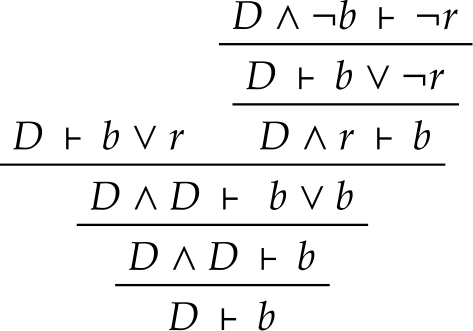
\includegraphics[width=1\textwidth,height=\textheight]{umbrella_inference_sequent.png}

}

\caption{The bottom formula is our conclusion; the formulae above it
represent steps in the proof. Each line denotes the application of an
inference rule. The two formulae with no line above are our two
assumptions.}

\end{marginfigure}

\hfill\break

We can compactly encode all inference rules in the following way. First,
represent \texttt{true} by the number \texttt{1}, and \texttt{false} by
\texttt{0}. Second, symbolically write that conclusion \(C\) is
\texttt{true}, given assumptions \(A\), as follows: \[
\mathrm{T}(C \nonscript\:\vert\nonscript\:\mathopen{} A) = 1 \ .
\] or with \texttt{0} if it's \texttt{false}.

The rules of truth inference are then encoded by the following
equations, which must always hold for any sentences \(A,B,C\), no matter
whether they are basic or complex:

\begin{figure*}

\begin{description}
\tightlist
\item[Rule for ``not'':]
\begin{equation}\protect\hypertarget{eq-t-not}{}{\mathrm{T}(\lnot A \nonscript\:\vert\nonscript\:\mathopen{} B) 
+ \mathrm{T}(A \nonscript\:\vert\nonscript\:\mathopen{} B)
= 1}\label{eq-t-not}\end{equation}
\item[Rule for ``and'':]
\begin{equation}\protect\hypertarget{eq-t-and}{}{
\mathrm{T}(A \land B \nonscript\:\vert\nonscript\:\mathopen{} C) 
= \mathrm{T}(A \nonscript\:\vert\nonscript\:\mathopen{} B \land C) \cdot
\mathrm{T}(B \nonscript\:\vert\nonscript\:\mathopen{} C) 
= \mathrm{T}(B \nonscript\:\vert\nonscript\:\mathopen{} A \land C) \cdot
\mathrm{T}(A \nonscript\:\vert\nonscript\:\mathopen{} C)
}\label{eq-t-and}\end{equation}
\item[Rule for ``or'':]
\begin{equation}\protect\hypertarget{eq-t-or}{}{\mathrm{T}(A \lor B \nonscript\:\vert\nonscript\:\mathopen{} C) 
= \mathrm{T}(A \nonscript\:\vert\nonscript\:\mathopen{} C) +
\mathrm{T}(B \nonscript\:\vert\nonscript\:\mathopen{} C) 
- \mathrm{T}(A \land B \nonscript\:\vert\nonscript\:\mathopen{} C)
}\label{eq-t-or}\end{equation}
\item[Rule of self-consistency:]
\begin{equation}\protect\hypertarget{eq-t-unity}{}{\mathrm{T}(A \nonscript\:\vert\nonscript\:\mathopen{} A \land C) 
= 1
}\label{eq-t-unity}\end{equation}
\end{description}

\end{figure*}

\hfill\break

Let's see how the inference rule (\textbf{?@eq-example-rule}), for
example, is encoded in these equations. The rule starts with saying that
\(a \land b\) is \texttt{true} according to \(D\). This means that
\(\mathrm{T}(a \land b \nonscript\:\vert\nonscript\:\mathopen{} D)=1\).
But, by rule (\ref{eq-t-and}), we must then have
\(\mathrm{T}(b \nonscript\:\vert\nonscript\:\mathopen{} a \land D) \cdot \mathrm{T}(a \nonscript\:\vert\nonscript\:\mathopen{} D) = 1\).
This can only happen if both
\(\mathrm{T}(b \nonscript\:\vert\nonscript\:\mathopen{} a \land D)\) and
\(\mathrm{T}(a \nonscript\:\vert\nonscript\:\mathopen{} D)\) are equal
to \(1\). So we can conclude that
\(\mathrm{T}(a \nonscript\:\vert\nonscript\:\mathopen{} D)=1\), which is
exactly the conclusion under the line in rule
(\textbf{?@eq-example-rule}).

\begin{tcolorbox}[enhanced jigsaw, opacityback=0, colback=white, toprule=.15mm, left=2mm, colframe=quarto-callout-caution-color-frame, title={\faIcon{user-edit} Exercise}, colbacktitle=quarto-callout-caution-color!10!white, leftrule=.75mm, rightrule=.15mm, opacitybacktitle=0.6, breakable, coltitle=black, bottomtitle=1mm, toptitle=1mm, titlerule=0mm, arc=.35mm, bottomrule=.15mm]

Try to prove our initial inference

\[
\frac{
(b \lor r) \land \lnot (b \land r) \nonscript\:\vert\nonscript\:\mathopen{} D
\qquad
\lnot r \nonscript\:\vert\nonscript\:\mathopen{} D
}{
b\nonscript\:\vert\nonscript\:\mathopen{} D
}
\]

using the basic rules (\ref{eq-t-not}, \ref{eq-t-and}, \ref{eq-t-or},
\ref{eq-t-unity}). Remember that you can use each rule as many times as
you like, and that there is not only one way of constructing a proof.

\end{tcolorbox}

\hypertarget{logical-ai-agents-and-their-limitations}{%
\section{Logical AI agents and their
limitations}\label{logical-ai-agents-and-their-limitations}}

The basic rules above are also the rules that a logical
artificial-intelligent agent should follow.

\begin{tcolorbox}[enhanced jigsaw, opacityback=0, colback=white, toprule=.15mm, left=2mm, colframe=quarto-callout-caution-color-frame, title={\faIcon{book} Reading}, colbacktitle=quarto-callout-caution-color!10!white, leftrule=.75mm, rightrule=.15mm, opacitybacktitle=0.6, breakable, coltitle=black, bottomtitle=1mm, toptitle=1mm, titlerule=0mm, arc=.35mm, bottomrule=.15mm]

\href{https://hvl.instructure.com/courses/25074/modules/items/660089}{Ch.~7
in \emph{Artificial Intelligence}}

\end{tcolorbox}

Many -- if not most -- inference problems that a data engineer must face
are, however, of the \emph{uncertain} kind: it is not possible to surely
infer the truth of some data, and the truth of some initial data may not
be known either. In the next chapter we shall see how to generalize the
logic rules to uncertain situations.

\begin{tcolorbox}[enhanced jigsaw, opacityback=0, colback=white, toprule=.15mm, left=2mm, colframe=quarto-callout-tip-color-frame, title={\faIcon{rocket} For the extra curious}, colbacktitle=quarto-callout-tip-color!10!white, leftrule=.75mm, rightrule=.15mm, opacitybacktitle=0.6, breakable, coltitle=black, bottomtitle=1mm, toptitle=1mm, titlerule=0mm, arc=.35mm, bottomrule=.15mm]

Our cursory visit of formal logic only showed a microscopic part of this
vast field. The study of logic rules continues still today, with many
exciting developments and applications. Feel free take a look at
\href{https://hvl.instructure.com/courses/25074/modules/items/661036}{\emph{Logic
in Computer Science}},
\href{https://hvl.instructure.com/courses/25074/modules/items/661146}{\emph{Mathematical
Logic for Computer Science}},
\href{https://plato.stanford.edu/archives/spr2023/entries/natural-deduction}{Natural
Deduction Systems in Logic}

\end{tcolorbox}

\hypertarget{probability-inference}{%
\chapter{Probability inference}\label{probability-inference}}

\providecommand{\ul}{\uline}
\renewcommand*{\|}[1][]{\nonscript\:#1\vert\nonscript\:\mathopen{}}
\providecommand*{\pr}[1]{\textsf{\small`#1'}}
\renewcommand*{\pr}[1]{\textsf{\small`#1'}}
\providecommand*{\prq}[1]{\textsf{\small #1}}
\renewcommand*{\prq}[1]{\textsf{\small #1}}
\providecommand{\se}[1]{\mathsfit{#1}}
\renewcommand{\se}[1]{\mathsfit{#1}}
\providecommand{\p}{\mathrm{p}}
\renewcommand{\p}{\mathrm{p}}
\renewcommand{\P}{\mathrm{P}}
\definecolor{quarto-callout-note-color}{HTML}{4477AA}
\definecolor{quarto-callout-note-color-frame}{HTML}{4477AA}
\definecolor{quarto-callout-important-color}{HTML}{AA3377}
\definecolor{quarto-callout-important-color-frame}{HTML}{AA3377}
\definecolor{quarto-callout-warning-color}{HTML}{EE6677}
\definecolor{quarto-callout-warning-color-frame}{HTML}{EE6677}
\definecolor{quarto-callout-tip-color}{HTML}{228833}
\definecolor{quarto-callout-tip-color-frame}{HTML}{228833}
\definecolor{quarto-callout-caution-color}{HTML}{CCBB44}
\definecolor{quarto-callout-caution-color-frame}{HTML}{CCBB44}

\hypertarget{when-truth-isnt-known-probability}{%
\section{When truth isn't known:
probability}\label{when-truth-isnt-known-probability}}

In most real-life and engineering situations we don't know the truth or
falsity of sentences and hypotheses that interest us. But this doesn't
mean that nothing can be said or done in such situations.

When we cross a busy city street we look left and right to check whether
any cars are approaching. We typically don't look up to check whether
something is falling from the sky. Yet, couldn't it be \texttt{false}
that cars are approaching? and couldn't it be \texttt{true} that
\href{https://www.aerotime.aero/articles/32818-cessna-door-falls-off-lands-in-parking-lot}{some
object is falling from the sky}? Of course both events are possible.
Then why do we look left and right, but not up?

The main reason\footnote{We shall see later that one more factor enters
  the explanation.} is that we \emph{believe strongly} that cars might
be approaching, \emph{believe very weakly} that some object might be
falling from the sky. In other words, we consider the first occurrence
to be very \emph{probable}; the second, extremely improbable.

We shall take the notion of \textbf{probability} as intuitively
understood (just as we did with the notion of truth). Terms equivalent
for ``probability'' are \emph{degree of belief}, \emph{plausibility},
\emph{credibility}.

\begin{tcolorbox}[enhanced jigsaw, opacityback=0, leftrule=.75mm, rightrule=.15mm, colback=white, breakable, left=2mm, colframe=quarto-callout-important-color-frame, bottomrule=.15mm, arc=.35mm, toprule=.15mm]

\textbf{}\vspace{2mm}

\faIcon{exclamation-circle} In technical discourse, \emph{likelihood}
means something different and is \emph{not} a synonym of
``probability'', as we'll explain later.

\end{tcolorbox}

Probabilities are quantified between \texttt{0} and \texttt{1}, or
equivalently between \texttt{0\%} and \texttt{100\%}. Assigning to a
sentence a probability \texttt{1} is the same as saying that it is
\texttt{true}; and a probability \texttt{0}, that it is \texttt{false}.
A probability of \texttt{0.5} represents a belief completely symmetric
with respect to truth and falsity.

It is important to emphasize and agree on some facts about
probabilities:

\begin{itemize}
\item
  \textbf{Probabilities are assigned to \emph{sentences}}. Consider an
  engineer working on a problem of electric-power distribution in a
  specific geographical region. At a given moment the engineer may
  believe with \texttt{75\%} probability that the measured average power
  output in the next hour will be 100~MW. The \texttt{75\%} probability
  is assigned not to the quantity ``100~MW'', but to the \emph{sentence}
  \[
  \textsf{\small`The measured average power output in the next hour will be 100\,MW'}
  \] This difference is extremely important. Consider the alternative
  sentence \[
  \textsf{\small`The average power output in the next hour will be \emph{set} to 100\,MW'}
  \] the quantity is the same, but the meaning is very different. The
  probability can therefore be very different (if the engineer is the
  person deciding the output, the probability is \texttt{100\%}). The
  probability depends not only on a number, but on what it's being done
  with that number -- measuring, setting, third-party reporting, and so
  on. Often we still write simply
  \(\textsf{\small`\(\mathsf{O = 100\,W}\)'}\) or even just
  \(\textsf{\small`100\,W'}\), provided that the full sentence behind
  the shorthand is understood.
\item
  \textbf{Probabilities are agent- and context-dependent}. A coin is
  tossed, comes down heads, and is quickly hidden from view. Alice sees
  that it landed heads-up. Bob instead doesn't manage to see the outcome
  and has no clue. Alice considers the sentence
  \(\textsf{\small`Coin came down heads'}\) to be \texttt{true}, that
  is, to have \texttt{100\%} probability. Bob considers the same
  sentence to have \texttt{50\%} probability.

  Note how Alice and Bob assign two different probabilities to the same
  sentence; yet both assignments are completely rational. If Bob
  assigned \texttt{100\%} to \(\textsf{\small`heads'}\), we would
  suspect that he had seen the outcome after all; if he assigned
  \texttt{0\%} to \(\textsf{\small`heads'}\), we would consider that
  groundless and silly. We would be baffled if Alice assigned
  \texttt{50\%} to \(\textsf{\small`heads'}\), because she saw the
  outcome was actually heads; we would hypothesize that she feels unsure
  about what she saw.

  An omniscient agent would know the truth or falsity of every sentence,
  and assign only probabilities \texttt{0} or \texttt{1}. Some authors
  speak of ``\emph{actual} (but unknown) probabilities''; if there were
  ``actual'' probabilities, they would be all \texttt{0} or \texttt{1},
  and it would be pointless to speak about probabilities at all -- every
  inference would be a truth inference.
\item
  \textbf{Probabilities are not frequencies}. The fraction of defective
  mechanical components to total components produced per year in some
  factory is a quantity that can be physically measured and would be
  agreed upon by every agent. It is a \emph{frequency}, not a degree of
  belief or probability. It is important to understand the difference
  between them, to avoid making sub-optimal decisions; we shall say more
  about this difference later. Frequencies can be unknown to some
  agents, probabilities cannot be unknown (but can be difficult to
  calculate). Be careful when you read authors speaking of an ``unknown
  probability''; either they actually mean ``unknown frequency'', or a
  probability that has to be calculated (it's ``unknown'' in the same
  sense that the value of \(1-0.7 \cdot 0.2/(1-0.3)\) is unknown to you
  right now).
\item
  \textbf{Probabilities are not physical properties}. Whether a tossed
  coin lands heads up or tails up is fully determined by the initial
  conditions (position, orientation, momentum, rotational momentum) of
  the toss and the boundary conditions (air velocity and pressure)
  during the flight. The same is true for all macroscopic engineering
  phenomena (even quantum phenomena have never been proved to be
  non-deterministic, and there are
  \href{https://doi.org/10.48550/arXiv.quant-ph/9504010}{deterministic
  and experimentally consistent} mathematical representations of quantum
  theory). So we cannot measure a probability using some physical
  apparatus; and the mechanisms underlying any engineering problem boil
  down to physical laws, not to probabilities.
\end{itemize}

\begin{tcolorbox}[enhanced jigsaw, opacityback=0, colback=white, toprule=.15mm, left=2mm, colframe=quarto-callout-caution-color-frame, title={\faIcon{book} Reading}, colbacktitle=quarto-callout-caution-color!10!white, leftrule=.75mm, rightrule=.15mm, opacitybacktitle=0.6, breakable, coltitle=black, bottomtitle=1mm, toptitle=1mm, titlerule=0mm, arc=.35mm, bottomrule=.15mm]

\href{https://hvl.instructure.com/courses/25074/modules/items/661553}{\emph{Dynamical
Bias in the Coin Toss}}

\end{tcolorbox}

These facts are not just a matter of principle. They have important
practical consequences. A data engineer who is not attentive to the
source of the data (measured? set? reported, and so maybe less
trustworthy?), or who does not carefully assess the context of a
probability, or who mixes it up with something else, or who does not
take advantage (when possible) of the physics involved in the
engineering problem, will design a system with sub-optimal
performance\footnote{This fact can be mathematically proven.} -- or even
cause deaths.

\hypertarget{no-new-building-blocks}{%
\section{No new building blocks}\label{no-new-building-blocks}}

In discussing \protect\hyperlink{sec-truth-inference}{truth-inference}
we introduced notations such as
\(\mathrm{T}(a \nonscript\:\vert\nonscript\:\mathopen{} b \land D)\),
which stands for the truth-value \texttt{0} or \texttt{1} of sentence
\(a\) in the context of data \(D\) and supposing (even if only
hypothetically) sentence \(b\) to be true. We can simply extend this
notation to probability-values, using a \(\mathrm{P}\) instead of
\(\mathrm{T}\):
\[\mathrm{P}(a \nonscript\:\vert\nonscript\:\mathopen{} b \land D) \in [0,1]\]
represents the probability or degree of belief in sentence \(a\) in the
context of data \(D\) and supposing also sentence \(b\) to be true. Keep
in mind that both \(a\) and \(b\) could be complex sentences (for
instance \(a = (\lnot c \lor d) \land e\)). Note that truth-values are
included as the special cases\texttt{1} or \texttt{0}: \[
\mathrm{P}(a \nonscript\:\vert\nonscript\:\mathopen{} b \land D) = 0\text{ or }1
\quad\Longleftrightarrow\quad
\mathrm{T}(a \nonscript\:\vert\nonscript\:\mathopen{} b \land D) = 0\text{ or }1
\]

\hypertarget{probability-inference-rules}{%
\section{Probability-inference
rules}\label{probability-inference-rules}}

Extending our truth-inference notation to probability-inference notation
has been straightforward. But how do we draw inferences when
probabilities are involved?

Consider the inference about my umbrella in a more uncertain situation:

\begin{figure*}

\[
\frac{
\mathrm{P}(\textsf{\small`My umbrella is either blue or red'}\nonscript\:\vert\nonscript\:\mathopen{}D)=1\quad
\mathrm{P}(\textsf{\small`My umbrella is not red'} \nonscript\:\vert\nonscript\:\mathopen{} D)=0.5
}{
\mathrm{P}(\textsf{\small`My umbrella is blue'} \nonscript\:\vert\nonscript\:\mathopen{} D) = \mathord{?}
}
\]

\end{figure*}

or more compactly, using the symbols we introduced earlier, \[
\frac{
\mathrm{P}\bigl[(b \lor r) \land \lnot (b \land r)\nonscript\:\vert\nonscript\:\mathopen{}D\bigr]=1\quad
\mathrm{P}(\lnot r\nonscript\:\vert\nonscript\:\mathopen{} D)=0.5
}{
\mathrm{P}( b \nonscript\:\vert\nonscript\:\mathopen{} D) = \mathord{?}
}
\] This says, above the line, that: according to our data \(D\) my
umbrella is either blue or red (and can't be both), with full certainty;
and according to our data we have no preferential beliefs on whether my
umbrella is not red. What should then be the probability of my umbrella
being blue, according to our data?

Intuitively that probability should be \texttt{50\%}:
\(\mathrm{P}( b \nonscript\:\vert\nonscript\:\mathopen{} D)=0.5\). But
which rules did we follow in arriving at this probability? More
generally, which rules should we follow in assigning new probabilities
from given ones?

The amazing result is that \emph{the rules for truth-inference, formulae
(\ref{eq-t-not}, \ref{eq-t-or}, \ref{eq-t-and}, \ref{eq-t-unity}),
extend also to probability-inference}. The only difference is that they
now hold for all values in the range \([0,1]\), rather than only values
\(0\) and \(1\).

This important result was taken more or less for granted at least since
Laplace in the 1700s. But was formally proven for the first time in the
1940s by R.~T.~Cox; the proof has been refined since then. What kind of
proof is it? It shows that if we don't follow the rules we arrive at
illogical conclusions; we'll show some examples later.

Here are the fundamental rules of probability inference. In these rules,
all probabilities can have values in the range
\(\mathrm{P}() \in [0,1]\), and the symbols \(a,b,D\) represent
sentences of any complexity:

\begin{figure*}

\begin{tcolorbox}[enhanced jigsaw, opacityback=0, colback=white, toprule=.15mm, left=2mm, colframe=quarto-callout-note-color-frame, title={\faIcon{landmark}~~~THE FUNDAMENTAL LAWS OF
INFERENCE~~~\faIcon{landmark}}, colbacktitle=quarto-callout-note-color!10!white, leftrule=.75mm, rightrule=.15mm, opacitybacktitle=0.6, breakable, coltitle=black, bottomtitle=1mm, toptitle=1mm, titlerule=0mm, arc=.35mm, bottomrule=.15mm]

\begin{description}
\tightlist
\item[``Not'' \(\boldsymbol{\lnot}\) rule]
\[\mathrm{P}(\lnot a \nonscript\:\vert\nonscript\:\mathopen{} D) 
+ \mathrm{P}(a \nonscript\:\vert\nonscript\:\mathopen{} D)
= 1\]\\
\item[``And'' \(\boldsymbol{\land}\) rule]
\[
\mathrm{P}(a \land b \nonscript\:\vert\nonscript\:\mathopen{} D) 
= \mathrm{P}(a \nonscript\:\vert\nonscript\:\mathopen{} b \land D) \cdot
\mathrm{P}(b \nonscript\:\vert\nonscript\:\mathopen{} D) 
= \mathrm{P}(b \nonscript\:\vert\nonscript\:\mathopen{} a \land D) \cdot
\mathrm{P}(a \nonscript\:\vert\nonscript\:\mathopen{} D) 
\]\\
\item[``Or'' \(\boldsymbol{\lor}\) rule]
\[\mathrm{P}(a \lor b \nonscript\:\vert\nonscript\:\mathopen{} D) 
= \mathrm{P}(a \nonscript\:\vert\nonscript\:\mathopen{} D) +
\mathrm{P}(b \nonscript\:\vert\nonscript\:\mathopen{} D) 
- \mathrm{P}(a \land b \nonscript\:\vert\nonscript\:\mathopen{} D)
\]\\
\item[Self-consistency rule]
\[\mathrm{P}(a \nonscript\:\vert\nonscript\:\mathopen{} a \land D) 
= 1
\]
\end{description}

\end{tcolorbox}

\end{figure*}

It is amazing that \textbf{ALL} inference is nothing else but a repeated
application of these four rules -- billions of times or more, in some
inferences. All machine-learning algorithms are just applications or
approximations of these rules. Methods that you may have heard about in
statistics are just specific applications of these rules. Truth
inferences are also special applications of these rules. Most of this
course is, at bottom, just a study of how to apply these rules in
particular kinds of problems.

\begin{tcolorbox}[enhanced jigsaw, opacityback=0, colback=white, toprule=.15mm, left=2mm, colframe=quarto-callout-caution-color-frame, title={\faIcon{book} Reading}, colbacktitle=quarto-callout-caution-color!10!white, leftrule=.75mm, rightrule=.15mm, opacitybacktitle=0.6, breakable, coltitle=black, bottomtitle=1mm, toptitle=1mm, titlerule=0mm, arc=.35mm, bottomrule=.15mm]

\begin{itemize}
\item
  \href{https://hvl.instructure.com/courses/25074/modules/items/660094}{\emph{Probability,
  Frequency and Reasonable Expectation}}
\item
  Ch.~2 of
  \href{https://hvl.instructure.com/courses/25074/modules/items/660390}{\emph{Bayesian
  Logical Data Analysis for the Physical Sciences}}
\item
  §§~1.0--1.2 of
  \href{https://hvl.instructure.com/courses/25074/modules/items/661040}{\emph{Data
  Analysis}}
\item
  Feel free to skim through §§~2.0--2.4 of
  \href{https://hvl.instructure.com/courses/25074/modules/items/660090}{\emph{Probability
  Theory}}
\end{itemize}

\end{tcolorbox}

\hypertarget{how-the-inference-rules-are-used}{%
\section{How the inference rules are
used}\label{how-the-inference-rules-are-used}}

The fundamental rules represent, first of all, constraints of logical
consistency among probabilities. If we have probabilities
\(\mathrm{P}(a\nonscript\:\vert\nonscript\:\mathopen{}D)=0.7\),
\(\mathrm{P}(b\nonscript\:\vert\nonscript\:\mathopen{}a\land D)=0.1\),
\(\mathrm{P}(a\land b\nonscript\:\vert\nonscript\:\mathopen{}D)=0.2\),
then there's an inconsistency somewhere, because these values violate
the and-rule:~~\(0.2 \ne 0.1 \cdot 0.7\).~~In this case we must find the
inconsistency and solve it. Since probabilities are quantified by real
numbers, however, it's possible and acceptable to have slight
discrepancies owing to numerical round-off errors.

The rules also imply more general constraints. For example we must
\emph{always} have \begin{gather*}
\mathrm{P}(a\land b \nonscript\:\vert\nonscript\:\mathopen{}D) \le \min\bigl\{\mathrm{P}(a\nonscript\:\vert\nonscript\:\mathopen{}D),\  \mathrm{P}(b\nonscript\:\vert\nonscript\:\mathopen{}D)\bigr\}
\\
\mathrm{P}(a\lor b \nonscript\:\vert\nonscript\:\mathopen{}D) \ge \max\bigl\{\mathrm{P}(a\nonscript\:\vert\nonscript\:\mathopen{}D),\  \mathrm{P}(b\nonscript\:\vert\nonscript\:\mathopen{}D)\bigr\}
\end{gather*}

\begin{tcolorbox}[enhanced jigsaw, opacityback=0, colback=white, toprule=.15mm, left=2mm, colframe=quarto-callout-caution-color-frame, title={\faIcon{user-edit} Exercise}, colbacktitle=quarto-callout-caution-color!10!white, leftrule=.75mm, rightrule=.15mm, opacitybacktitle=0.6, breakable, coltitle=black, bottomtitle=1mm, toptitle=1mm, titlerule=0mm, arc=.35mm, bottomrule=.15mm]

Try to prove the two constraints above

\end{tcolorbox}

The main use of the rules in concrete applications is for calculating
new probabilities from given ones. The calculated probabilities will be
automatically consistent. For each equation shown in the rules we can
calculate one probability given the remaining ones in the equation, with
some special cases when values of \(0\) or \(1\) appear.

For example, if we have
\(\mathrm{P}(a \land b\nonscript\:\vert\nonscript\:\mathopen{} D)=0.2\)
and \(\mathrm{P}(a\nonscript\:\vert\nonscript\:\mathopen{}D)=0.7\), from
the and-rule we can find
\(\mathrm{P}(b\nonscript\:\vert\nonscript\:\mathopen{} a \land D)\):
\begin{multline*}
\underbracket{\color[RGB]{34,136,51}\mathrm{P}(a \land b \nonscript\:\vert\nonscript\:\mathopen{} D)}_{0.2}
= {\color[RGB]{238,102,119}\mathrm{P}(b \nonscript\:\vert\nonscript\:\mathopen{} a \land D)} \cdot
\underbracket{\color[RGB]{34,136,51}\mathrm{P}(a \nonscript\:\vert\nonscript\:\mathopen{} D)}_{0.7}
\\[1em]
\Longrightarrow\quad
{\color[RGB]{238,102,119}\mathrm{P}(b\nonscript\:\vert\nonscript\:\mathopen{} a \land D)} = 
\frac{\color[RGB]{34,136,51}
\mathrm{P}(a\land b \nonscript\:\vert\nonscript\:\mathopen{} D)
}{\color[RGB]{34,136,51}
\mathrm{P}(a\nonscript\:\vert\nonscript\:\mathopen{}D)
} = \frac{0.2}{0.7} 
\approx 0.2857
\end{multline*}\\

Let us now solve the umbrella inference from the previous section.
Starting from \[
\mathrm{P}\bigl[(b \lor r) \land \lnot (b \land r)\nonscript\:\vert\nonscript\:\mathopen{}D\bigr]=1 \ ,
\quad
\mathrm{P}(\lnot r\nonscript\:\vert\nonscript\:\mathopen{} D)=0.5
\] we arrive at \[
\mathrm{P}( b \nonscript\:\vert\nonscript\:\mathopen{} D) = 0.5
\]

by following from top to bottom the steps depicted here:

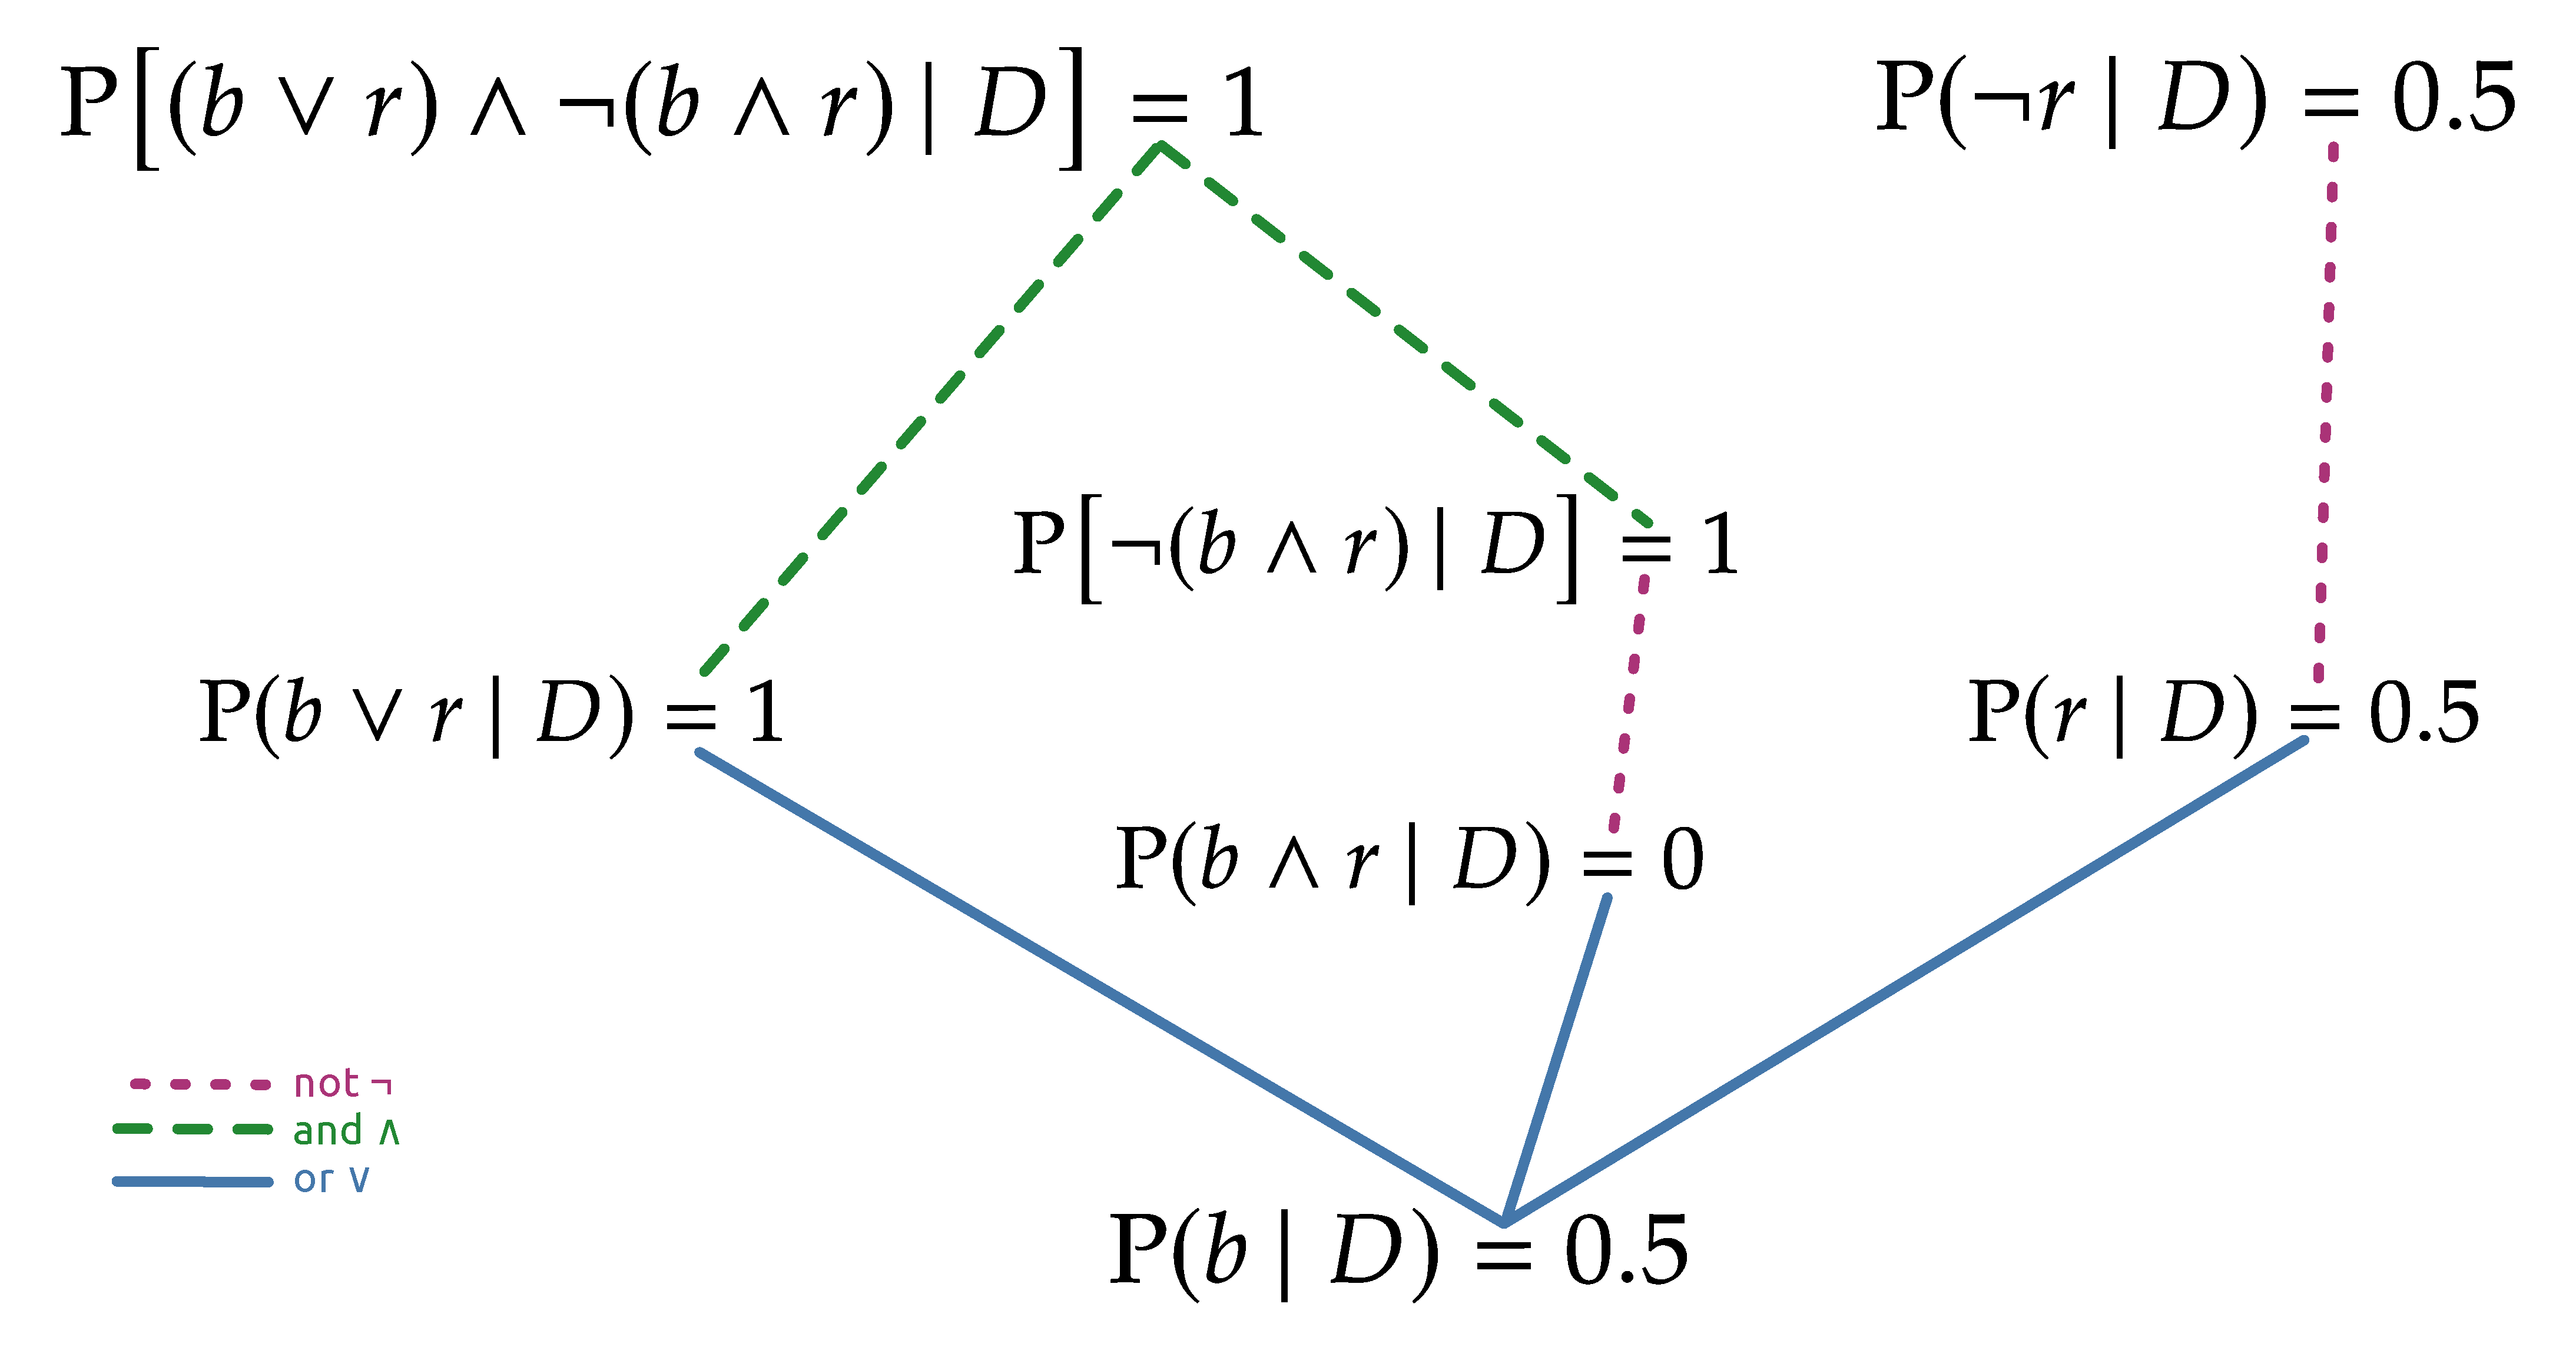
\includegraphics{index_files/mediabag/umbrella_inference2.pdf}

@@ example medical diagnosis

\hypertarget{derived-rules}{%
\subsection{Derived rules}\label{derived-rules}}

The rules above are in principle all we need to use. But from them it is
possible to derive some additional shortcut rules that are automatically
consistent with the fundamental ones.

First, it is possible to show that all rules you may know from Boolean
algebra are a consequence of the fundamental rules. For example, we can
always make the following convenient replacements anywhere in a
probability expression: \[
\begin{gathered}
A \land A = A \lor A = A
\qquad
\lnot\lnot A = A
\\[1ex]
A\land B = B \land A
\qquad
A \lor B = B \lor A
\\[1ex]
\lnot (A \land B) = \lnot A \lor \lnot B
\qquad
\lnot (A \lor B) = \lnot A \land \lnot B
\\[1ex]
A \land (B \lor C) = (A \land B) \lor (A \land C)
\\[1ex]
A \lor (B \land C) = (A \lor B) \land (A \lor C)
\end{gathered}
\]

Two other derived rules are used extremely often, so we treat them
separately.

\hypertarget{law-of-total-probability-or-extension-of-the-conversation}{%
\section{Law of total probability or ``extension of the
conversation''}\label{law-of-total-probability-or-extension-of-the-conversation}}

\hypertarget{bayess-theorem}{%
\section{Bayes's theorem}\label{bayess-theorem}}

\begin{marginfigure}

{\centering 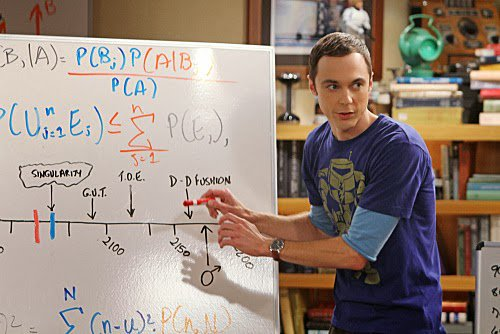
\includegraphics{bayes_big-bang.jpg}

}

\caption{Bayes's theorem guest-starring in
\href{https://www.imdb.com/title/tt0898266/}{\emph{The Big Bang
Theory}}}

\end{marginfigure}

\hypertarget{consequences-of-not-following-the-rules}{%
\section{consequences of not following the
rules,}\label{consequences-of-not-following-the-rules}}

@@ §12.2.3 of AI

\begin{itemize}
\item
  \emph{Exercise: \href{The_Monty_Hall_problem-exercise.pdf}{Monty-Hall
  problem \& variations}}
\item
  \emph{Exercise: clinical test \& diagnosis}
\end{itemize}

\hypertarget{common-points-of-certain-and-uncertain-inference}{%
\section{Common points of certain and uncertain
inference}\label{common-points-of-certain-and-uncertain-inference}}

\begin{quote}
\emph{No premises? No conclusions!}
\end{quote}

\begin{tcolorbox}[enhanced jigsaw, opacityback=0, colback=white, toprule=.15mm, left=2mm, colframe=quarto-callout-important-color-frame, title={\faIcon{exclamation-circle} Differences in terminology}, colbacktitle=quarto-callout-important-color!10!white, leftrule=.75mm, rightrule=.15mm, opacitybacktitle=0.6, breakable, coltitle=black, bottomtitle=1mm, toptitle=1mm, titlerule=0mm, arc=.35mm, bottomrule=.15mm]

\begin{itemize}
\item
  Some texts speak of the probability of a ``random\footnotemark{}
  variable'', or more precisely of the probability that a random
  variable takes on a particular value. As you notice, we have just
  expressed that idea by means of a \emph{sentence}. The viewpoint and
  terminology of random variables is a special case of that of
  sentences. As already discussed, in concrete applications it is
  important to know how a variable ``takes on'' a value: for example it
  could be directly measured, indirectly reported, or purposely set.
  Thinking in terms of sentences, rather than of random variables,
  allows us to account for these important differences.
\item
  Some texts speak of the probability of an ``event''. For all purposes
  an ``event'' is just what's expressed in a sentence.
\end{itemize}

It's a question for sociology of science why some people keep on using
less flexible points of view or terminologies. Probably they just
memorize them as students and then a fossilization process sets in.

\end{tcolorbox}

\footnotetext{What does ''random'' mean? Good luck finding an
understandable and non-circular definition in texts that use that word.
In these notes, if the word ''random'' is ever used, it means
''unpredictable'' or ''unsystematic''.}

\hypertarget{data-and-information}{%
\chapter{Data and information}\label{data-and-information}}

\hypertarget{kinds-of-data}{%
\section{Kinds of data}\label{kinds-of-data}}

\hypertarget{binary}{%
\subsection{Binary}\label{binary}}

\hypertarget{nominal}{%
\subsection{Nominal}\label{nominal}}

\hypertarget{ordinal}{%
\subsection{Ordinal}\label{ordinal}}

\hypertarget{continuous}{%
\subsection{Continuous}\label{continuous}}

\begin{itemize}
\item
  unbounded
\item
  bounded
\item
  censored
\end{itemize}

\hypertarget{complex-data}{%
\subsection{Complex data}\label{complex-data}}

2D, 3D, images, graphs, etc.

\hypertarget{soft-data}{%
\subsection{``Soft'' data}\label{soft-data}}

\begin{itemize}
\item
  orders of magnitude
\item
  physical bounds
\end{itemize}

\hypertarget{data-transformations}{%
\section{Data transformations}\label{data-transformations}}

\begin{itemize}
\item
  log
\item
  probit
\item
  logit
\end{itemize}

\hypertarget{allocation-of-uncertainty-among-possible-data-values-probability-distributions}{%
\chapter{Allocation of uncertainty among possible data values:
probability
distributions}\label{allocation-of-uncertainty-among-possible-data-values-probability-distributions}}

\hypertarget{the-difference-between-statistics-and-probability-theory}{%
\section{The difference between Statistics and Probability
Theory}\label{the-difference-between-statistics-and-probability-theory}}

\emph{Statistics} is the study of collective properties of collections
of data. It does not imply that there is any uncertainty.

\emph{Probability theory} is the quantification and propagation of
uncertainty. It does not imply that we have collections of data.

\hypertarget{whats-distributed}{%
\section{What's ``distributed''?}\label{whats-distributed}}

Difference between distribution of probability and distribution of (a
collection of) data.

\hypertarget{distributions-of-probability}{%
\section{Distributions of
probability}\label{distributions-of-probability}}

\hypertarget{representations}{%
\subsection{Representations}\label{representations}}

\begin{itemize}
\item
  Density function
\item
  Histogram
\item
  Scatter plot
\end{itemize}

Behaviour of representations under transformations of data.

\hypertarget{summaries-of-distributions-of-probability}{%
\section{Summaries of distributions of
probability}\label{summaries-of-distributions-of-probability}}

\hypertarget{location}{%
\subsection{Location}\label{location}}

Median, mean

\hypertarget{dispersion-or-range}{%
\subsection{Dispersion or range}\label{dispersion-or-range}}

Quantiles \& quartiles, interquartile range, median absolute deviation,
standard deviation, half-range

\hypertarget{resolution}{%
\subsection{Resolution}\label{resolution}}

Differential entropy

\hypertarget{behaviour-of-summaries-under-transformations-of-data-and-errors-in-data}{%
\subsection{Behaviour of summaries under transformations of data and
errors in
data}\label{behaviour-of-summaries-under-transformations-of-data-and-errors-in-data}}

\hypertarget{outliers-and-out-of-population-data}{%
\section{Outliers and out-of-population
data}\label{outliers-and-out-of-population-data}}

(Warnings against tail-cutting and similar nonsense-practices)

\hypertarget{marginal-and-conditional-distributions-of-probability}{%
\section{Marginal and conditional distributions of
probability}\label{marginal-and-conditional-distributions-of-probability}}

\hypertarget{collecting-and-sampling-data}{%
\section{Collecting and sampling
data}\label{collecting-and-sampling-data}}

\hypertarget{representative-samples}{%
\subsection{``Representative'' samples}\label{representative-samples}}

Size of minimal representative sample = (2\^{}entropy)/precision

\begin{itemize}
\tightlist
\item
  \emph{Exercise: data with 14 binary variates, 10000 samples}
\end{itemize}

\hypertarget{unavoidable-sampling-biases}{%
\subsection{Unavoidable sampling
biases}\label{unavoidable-sampling-biases}}

In high dimensions, all datasets are outliers.

Data splits and cross-validation cannot correct sampling biases

\hypertarget{quirks-and-warnings-about-high-dimensional-data}{%
\section{Quirks and warnings about high-dimensional
data}\label{quirks-and-warnings-about-high-dimensional-data}}

\hypertarget{making-decisions}{%
\chapter{Making decisions}\label{making-decisions}}

\hypertarget{decisions-possible-situations-and-consequences}{%
\section{Decisions, possible situations, and
consequences}\label{decisions-possible-situations-and-consequences}}

\hypertarget{gains-and-losses-utilities}{%
\section{Gains and losses: utilities}\label{gains-and-losses-utilities}}

\hypertarget{factors-that-enter-utility-quantification}{%
\subsection{Factors that enter utility
quantification}\label{factors-that-enter-utility-quantification}}

Utilities can rarely be assigned a priori.

\hypertarget{making-decisions-under-uncertainty-maximization-of-expected-utility}{%
\section{Making decisions under uncertainty: maximization of expected
utility}\label{making-decisions-under-uncertainty-maximization-of-expected-utility}}

\hypertarget{the-most-general-inference-problem}{%
\chapter{The most general inference
problem}\label{the-most-general-inference-problem}}



\end{document}
